\documentclass[conference]{IEEEtran}
\IEEEoverridecommandlockouts

\usepackage{cite}
\usepackage{amsmath,amssymb,amsfonts}
\usepackage{algorithmic}
\usepackage{algorithm}
\usepackage{graphicx}
\usepackage{textcomp}
\usepackage{xcolor}
\usepackage{enumitem}
\usepackage{booktabs}
\usepackage{multirow}
\def\BibTeX{{\rm B\kern-.05em{\sc i\kern-.025em b}\kern-.08em
    T\kern-.1667em\lower.7ex\hbox{E}\kern-.125emX}}

\begin{document}

\title{Trust-Based Governance for Fault-Resilient Multi-Agent Frontier
Exploration: The REIP Framework}

\author{\IEEEauthorblockN{William R. Kollmyer}
\IEEEauthorblockA{\textit{Olympia High School}\\
Olympia, Washington, USA\\
rykerkollmyer@gmail.com}}

\maketitle

%=========================================================================
\begin{abstract}
%=========================================================================
This paper introduces the Resilient Election and Impeachment Policy
(REIP), a trust-governed controller for fault-resilient hierarchical
multi-agent frontier exploration.  REIP enables agents to elect, monitor,
and impeach their leader without centralized oversight through a
distributed trust ledger and democratic governance protocol.  We present
two trust models: (i)~a \emph{reactive} model using CUSUM--Bayesian
fault detection, validated in 2\,000-seed GridWorld trials; and
(ii)~a \emph{proactive} three-tier confidence-weighted model where agents
verify commands \emph{before execution} against local knowledge ranked by
source reliability.  The proactive model provides a worst-case detection
bound of $\lceil \sigma / (w_{\min} - r) \rceil$ commands (2~under
ground truth, 8~under peer evidence).  A novel command stability metric
$\Omega$ classifies the fault type---persistent vs.\ oscillating
Byzantine behavior---from the angular velocity of the commanded
direction alone.  In GridWorld, REIP raises adversarial coverage from
22.0\% to 98.0\% ($+76\,$pp).  In multiroom evaluation with dual
sequential Byzantine fault injection ($N{=}100$ trials $\times$
9~conditions), REIP achieves 100\% median coverage under both clean and
adversarial conditions, detecting faults in $0.21 \pm 0.06\,$s---a
$+32.3\,$pp mean coverage advantage over Raft consensus, which cannot
detect a misbehaving leader that maintains heartbeats.  Hardware
validation on a five-robot platform with overhead ArUco localization
confirms sub-second fault detection without executing bad commands.
\end{abstract}

\begin{IEEEkeywords}
multi-agent systems, frontier exploration, trust governance, resilient
robotics, autonomous swarms, distributed fault detection
\end{IEEEkeywords}

%=========================================================================
\section{Introduction}
%=========================================================================

\subsection{Motivation and Context}
Multi-agent exploration teams enable surface mapping, disaster-response
surveys, and autonomous inspection missions faster than single robots can
achieve alone~\cite{yamauchi1997frontier, burgard2000collaborative}.
Hierarchical leader--follower coordination remains attractive because a
designated leader can allocate frontiers, manage conflicts, and exploit a
global view of the team's belief state, improving task efficiency over
purely decentralized swarms~\cite{burgard2000collaborative,
simmons2000coordination}.  However, leader--follower architectures
introduce a single point of failure: sensor faults, adversarial
interference, and AI-generated hallucinations can propagate system-wide
through the leader's commands~\cite{douceur2002sybil,
ji2023hallucination}.

\subsection{Problem Statement}
When a leader is compromised---through sensor degradation, adversarial
attack, or hallucinatory overconfidence---traditional control loops lack
mechanisms to detect and recover from compromised leadership.  Round-robin
rotation policies can reinstate faulty agents, and Byzantine fault-tolerant
(BFT) protocols require reliable all-to-all communication and honest
supermajorities rarely achievable in bandwidth-limited robotic
teams~\cite{lamport1982byzantine, castro1999practical}.  Frontier-based
exploration strategies assume agents act in good
faith~\cite{yamauchi1997frontier, burgard2000collaborative}, and trust
frameworks are seldom coupled with concrete impeachment policies for
robotic swarms~\cite{marsh1994formalising}.

A further gap separates simulation-validated governance from real-world
deployment.  Reactive trust models that measure performance \emph{after}
commands are followed introduce detection latency that wastes physical
time and energy.  Real-time hardware deployment demands \emph{proactive}
verification of leader commands before execution.

\subsection{Proposed Solution}
This paper proposes the Resilient Election and Impeachment Policy (REIP),
a trust-based governance framework for distributed multi-agent systems.
REIP combines per-agent fault detection, democratic leader impeachment,
and trust-based leader election without requiring centralized oversight or
ground-truth oracle access.

We present two trust models reflecting the system's iterative
development:
\begin{enumerate}
    \item A \textbf{reactive model} that monitors coverage prediction
    error using hybrid CUSUM--Bayesian fault
    detection~\cite{page1954cusum, gelman2013bayesian}, validated across
    2\,000 seeded GridWorld trials (Section~\ref{sec:gridworld}).
    \item A \textbf{proactive model} that verifies leader commands
    against local knowledge using three-tier confidence-weighted suspicion
    accumulation.  This model is used in both the multiroom simulation
    experiments (Section~\ref{sec:multiroom}) and the hardware platform,
    running identical code on Raspberry Pi Zero~2W nodes.
\end{enumerate}

The transition from reactive to proactive trust was motivated by
deployment realism: robots cannot afford to follow bad commands and then
measure the resulting damage.  The proactive model checks commands
against local belief \emph{before execution}, enabling sub-second fault
detection in both simulation and hardware.

\subsection{Contributions}
\begin{enumerate}
    \item A trust-based governance framework enabling distributed fault
    detection and democratic impeachment in multi-agent exploration
    without ground-truth oracle access.
    \item A reactive trust model using coverage prediction error with
    CUSUM--Bayesian fault detection, validated in large-scale GridWorld
    simulation.
    \item A proactive three-tier confidence-weighted trust model that
    verifies commands before execution, validated in multiroom
    simulation and deployed on embedded hardware, with a
    closed-form worst-case detection bound.
    \item A causality-aware verification mechanism that prevents false
    positives from concurrent exploration by timestamping visited cells
    against leader assignment times.
    \item A command stability metric $\Omega$ that automatically
    classifies Byzantine leadership faults by type (persistent
    assignment vs.\ oscillation) using only the angular velocity of
    commanded directions---enabling differentiated recovery strategies.
    \item Ablation experiments demonstrating that governance and fallback
    autonomy are complementary---neither alone achieves the resilience of
    the combined system.
    \item Rigorous hardware-equivalent validation with $N{=}100$ trials
    per condition (900 total experiments), comparing REIP against Raft
    consensus and decentralized baselines under dual sequential Byzantine
    fault injection, with a dual-vector visualization methodology for
    post-processing analysis.
    \item Hardware validation on a five-robot distributed platform with
    overhead ArUco-based localization, compared against decentralized
    and Raft-style baselines.
\end{enumerate}

\subsection{Paper Organization}
Section~II reviews related work.  Section~III presents the system
architecture.  Section~IV describes the REIP methodology including both
trust models.  Section~V presents GridWorld simulation experiments.
Section~VI presents hardware-equivalent multiroom experiments with
$N{=}100$ trials.  Section~VII describes hardware validation.
Section~VIII discusses implications, and Section~IX concludes.

%=========================================================================
\section{Background and Related Work}
%=========================================================================

REIP lies at the intersection of Byzantine fault tolerance, multi-robot
frontier exploration, and trust-based coordination.  We review each area
and identify the gap that motivates our approach.

\subsection{Byzantine Fault Tolerance and Distributed Governance}
Classical BFT protocols provide strong guarantees against arbitrary faults
under assumptions of reliable communication and honest
supermajorities~\cite{lamport1982byzantine}.  Practical protocols such as
PBFT relax some synchrony assumptions~\cite{castro1999practical}, and
consensus algorithms such as Raft provide leader election and log
replication for crash-tolerant distributed
systems~\cite{ongaro2014raft}.  However, these approaches typically
assume dense communication graphs or reliable message delivery that are
difficult to realize in range-limited robot teams.

REIP adopts the spirit of BFT---explicitly modeling faulty leaders and
governing their authority---but operates under partial observability and
lossy communication.  Unlike Raft, which detects leader failure only via
heartbeat timeout~\cite{ongaro2014raft}, REIP incorporates task-level
performance reasoning into its leader assessment.  This distinction is
critical for robotic systems: a leader that is alive and communicating
but issuing degraded commands (e.g., from sensor hallucination) will
never trigger Raft's timeout-based detection, leaving the team under
indefinite faulty leadership.

\subsection{Multi-Robot Frontier Exploration}
Frontier-based exploration assigns robots to boundaries between known and
unknown space~\cite{yamauchi1997frontier}, with multi-robot extensions
coordinating assignments to increase coverage
rate~\cite{burgard2000collaborative}.  Leader--follower architectures
exploit a global view for coordinated
assignment~\cite{simmons2000coordination}, but treat the leader as
implicitly trustworthy.  There is no mechanism for detecting when the
leader becomes degraded, nor for replacing it without external
supervision.  REIP augments a standard frontier-based leader--follower
stack with a governance layer that monitors, impeaches, and replaces a
failing leader based on observed performance.

\subsection{Trust and Reputation in Multi-Agent Systems}
Trust frameworks quantify agent reliability from past
behavior~\cite{marsh1994formalising}, but often assume access to
ground-truth outcomes.  In multi-robot exploration under partial
observability, ground truth is not directly available; agents observe only
local coverage changes and peer broadcasts.  REIP implements a
belief-only trust ledger that operates without an oracle map or
centralized evaluator.  An early reactive variant drives trust from
coverage prediction error (Section~\ref{sec:sim_trust}); the current
proactive model verifies leader commands against local knowledge before
execution (Section~\ref{sec:hw_trust}), used in both multiroom
simulation and hardware deployment.

\subsection{Proactive vs.\ Reactive Fault Detection}
Most fault detection in multi-agent systems is
reactive~\cite{chandola2009anomaly}: anomalies are detected after
performance degrades.  Residual-based detectors monitor prediction errors
post-execution, introducing latency between fault onset and detection.
In physical robotic systems, this latency wastes movement, energy, and
mission time.  Proactive approaches that verify commands \emph{before}
execution are rare in multi-robot governance literature.  REIP's proactive
trust model contributes such a mechanism, where agents check leader
commands against locally verifiable knowledge before committing to
execution.

%=========================================================================
\section{System Architecture}
%=========================================================================

REIP operates as a governance layer atop a frontier-based leader--follower
exploration stack.  We describe both simulation and hardware
architectures.

\subsection{Layered Design}
The system operates on three layers:
\begin{enumerate}
    \item \textbf{Agent Knowledge Layer}: Each agent maintains a
    high-resolution local map of personally observed cells, a
    low-resolution global belief map aggregated from peer broadcasts, and
    a coverage/motion history.
    \item \textbf{Communication Layer}: Agents share compressed belief
    updates within communication range via peer-to-peer broadcast.
    \item \textbf{Governance Layer}: A distributed trust ledger and
    democratic impeachment/election protocol that determine leadership.
\end{enumerate}

The distinction between local and global maps is central to the hardware
trust model (Section~\ref{sec:hw_trust}): agents treat personal
observations as ground truth and peer-reported data as lower-confidence
evidence.

\begin{figure}[t]
\centering
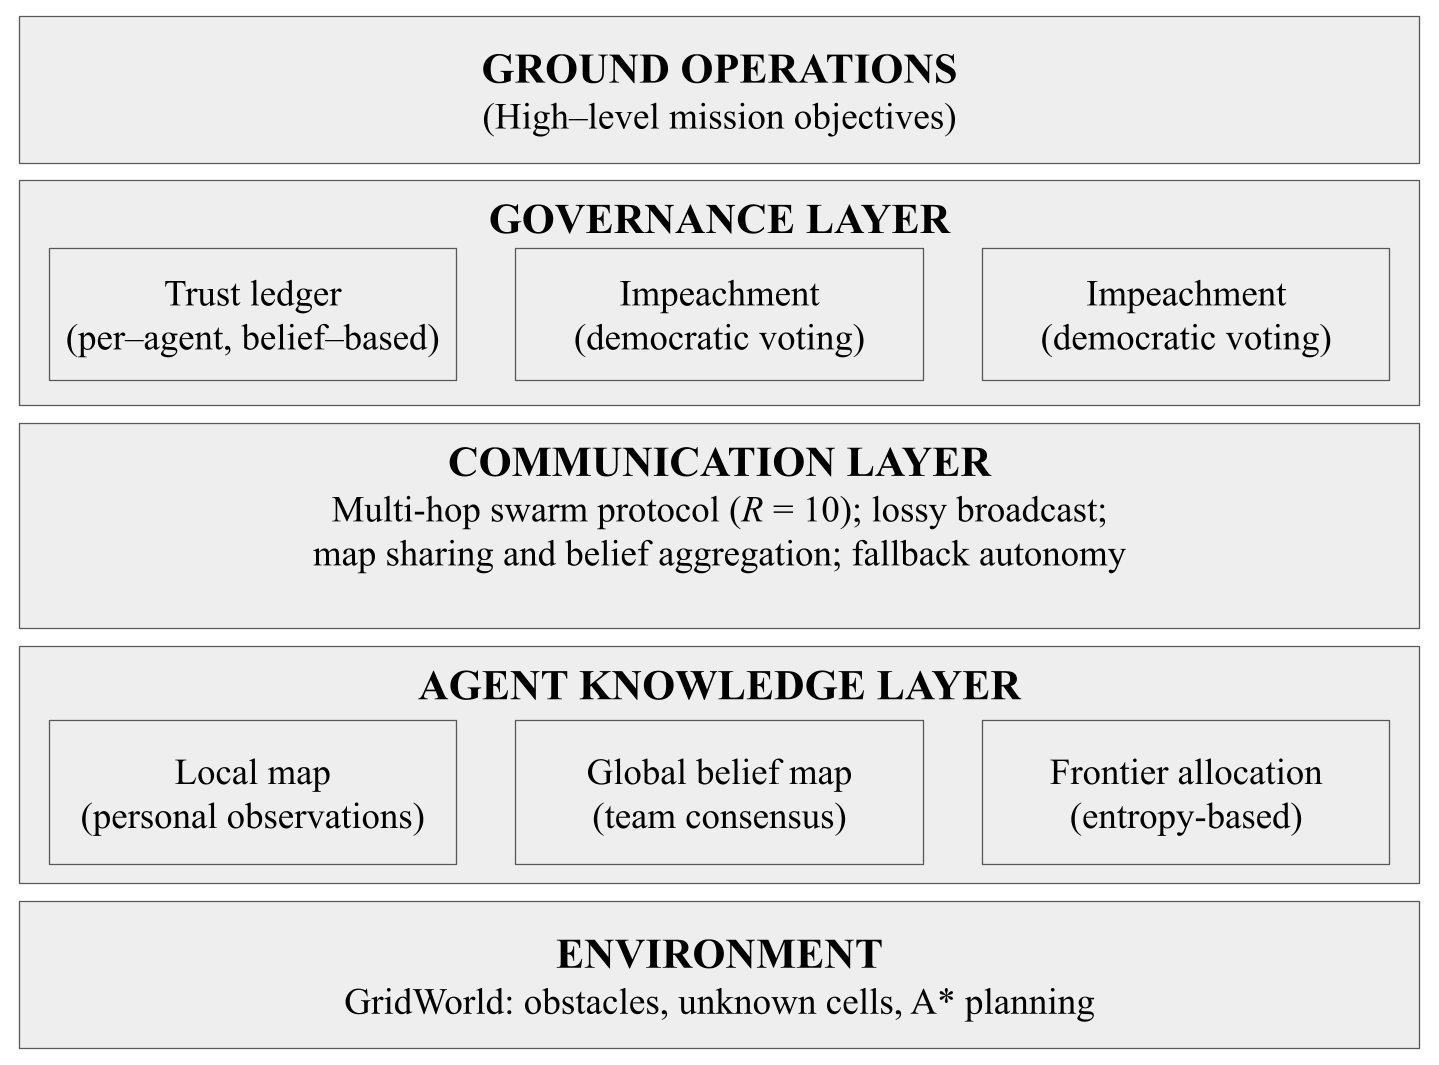
\includegraphics[width=\columnwidth]{flowfinal.png}
\caption{REIP system architecture.  The governance layer maintains a
per-agent trust ledger, impeachment protocol, and merit-based election.
The communication layer handles lossy peer-to-peer broadcast and belief
aggregation.  The agent knowledge layer separates high-resolution
personal observations from low-resolution peer-reported beliefs.
Fallback autonomy maintains exploration during leadership transitions.}
\label{fig:reip_arch}
\end{figure}

\subsection{Simulation Environment}
The simulation uses a 2D GridWorld with $60 \times 60$ cells, configurable
obstacle density, and deterministic map seeds for repeatable benchmarks.
Each agent has line-of-sight sensing (radius $r = 8$ cells) and
range-limited communication (radius $R$) with configurable packet loss
and corruption probabilities.  Path planning uses A* on the team belief
map without oracle access to ground truth~\cite{hart1968formal}.

For hardware-equivalent experiments (Section~\ref{sec:hw_sim}), a
physics-based harness simulates a $2000 \times 1500\,$mm arena with
$125\,$mm grid cells ($16 \times 12 = 192$ cells) and interior wall
segments.  Robot processes run the full REIP/Raft node software and
communicate via UDP, identical to hardware deployment.

\begin{figure}[t]
\centering
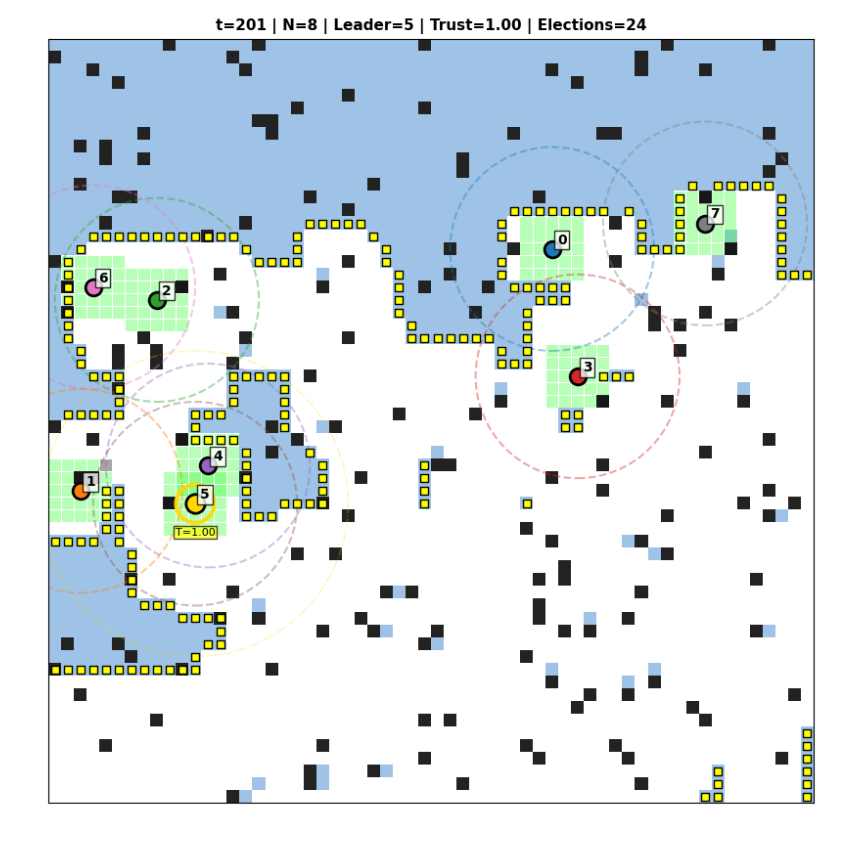
\includegraphics[width=\columnwidth]{gridworld.png}
\caption{GridWorld simulation environment.  Each dot is a numbered agent;
$N$ is the number of agents; $t$ is the current timestep; dotted circles
show communication radius; green circles show field of view; yellow halo
indicates leadership status.}
\label{fig:gridworld}
\end{figure}

\subsection{Hardware Platform}
\label{sec:hw_arch}
The hardware platform consists of five custom-built differential-drive
robots ($147 \times 111 \times 42\,$mm, $86.5\,$mm wheelbase) operating
in a $2000 \times 1500\,$mm arena partitioned into a virtual grid of
$125\,$mm cells ($16 \times 12 = 192$ cells).  Each robot is built
around a Raspberry Pi Zero 2W running the REIP node software, with a
Raspberry Pi Pico handling low-level motor control via UART.  Drive is
provided by two N20 geared DC motors (1:100 ratio) with magnetic
encoders, and a rear ball caster for stability.  Each robot carries five
VL53L0X time-of-flight (ToF) sensors on a TCA9548A I2C multiplexer,
providing $200\,$mm range obstacle detection.

Table~\ref{tab:bom} lists the per-robot bill of materials; total
platform cost including the shared overhead camera is approximately
\$514.

\begin{table}[h]
\centering
\caption{Per-Robot Bill of Materials}
\label{tab:bom}
\begin{tabular}{lcc}
\hline
\textbf{Component} & \textbf{Qty} & \textbf{Unit \$} \\
\hline
Raspberry Pi Zero 2W          & 1 & 15.00 \\
Raspberry Pi Pico H           & 1 &  5.00 \\
N20 Motor w/ Encoder (1:100)  & 2 &  4.50 \\
Pololu D30V30F5 5V Regulator  & 1 & 14.95 \\
VL53L0X ToF Sensor            & 5 &  2.60 \\
TCA9548A I2C Multiplexer      & 1 &  1.67 \\
Pololu 1/2'' Ball Caster      & 1 &  2.95 \\
N20 Rubber Wheels (3mm D)     & 2 &  2.00 \\
2S LiPo 7.4V 1000mAh         & 1 &  8.50 \\
32GB microSD Card             & 1 &  6.99 \\
3D-Printed Chassis (~60g PLA) & 1 &  3.00 \\
\hline
\textbf{Per robot}            &   & \textbf{\$84.56} \\
\hline
\end{tabular}
\end{table}

Localization is provided by an overhead camera (Logitech C922 at 1080p,
30\,fps) running ArUco marker detection~\cite{garrido2014aruco} on a
separate PC.  The PC acts
solely as a localization service: it detects each robot's ArUco marker,
computes pose $(x, y, \theta)$ in arena coordinates via a four-corner
homography transform using dedicated corner markers at the arena
boundaries, and transmits each robot's position via UDP broadcast.  The
PC has no knowledge of coverage state, leadership, trust, or task
assignments.

All coordination is fully distributed:
\begin{itemize}
    \item Robots broadcast state to peers via UDP at 5\,Hz;
    \item Each robot maintains its own visited-cell set and merges peer
    broadcasts into a shared coverage belief;
    \item Leadership election, trust assessment, and impeachment execute
    locally on each robot;
    \item The leader computes and broadcasts frontier assignments;
    followers verify assignments using the proactive three-tier trust
    model (Section~\ref{sec:hw_trust}).
\end{itemize}

\subsection{REIP Controller Decomposition}
The REIP controller comprises two complementary submodules:

\noindent\textbf{Governance} maintains a trust assessment module
(reactive in GridWorld, proactive in multiroom and hardware), merit-based
leader election, democratic impeachment, and peer anomaly detection that
monitors non-leader agents for behavioral faults (spinning, stuck,
coverage stall) to prevent compromised agents from inheriting leadership.

\noindent\textbf{Governed fallback} allows followers to revert to local
frontier exploration when trust in the leader drops below a threshold.
Governance determines \emph{when} to fall back; fallback provides the
safe behavior \emph{during} leadership transitions.  Without governance,
agents have no principled mechanism for deciding when to ignore the
leader.  Without fallback, governance can detect faults but agents have
no safe behavior to execute.  The two components are complementary:
governance is the trigger, fallback is the safety net.

%=========================================================================
\section{REIP Methodology}
%=========================================================================

\subsection{Reactive Trust Model (GridWorld)}
\label{sec:sim_trust}

The reactive trust model, used in the GridWorld experiments
(Section~\ref{sec:gridworld}), monitors the gap between predicted and
observed coverage gain.  For follower~$i$:
\begin{equation}
    T_i(t{+}1) = \max\!\bigl(T_{\min},\;
    \min\bigl(1,\; T_i(t)\,e^{-k\,\Delta U_t}\bigr)\bigr)
    \label{eq:trust_decay}
\end{equation}
with decay rate $k = 0.5$ and gated residual
\begin{equation}
    \Delta U_t = \max\bigl\{0,\;\bigl(U_{\text{pred}} -
    U_{\text{obs}}\bigr) - \delta\bigr\}
\end{equation}
where $\delta$ is a deadband that suppresses decay from routine noise.
A drop cap limits maximum trust loss per step.  Non-leader agents recover
trust toward 1.0 at rate~$\rho$:
\begin{equation}
    T_{ij}(t{+}1) = \min\bigl(1,\; T_{ij}(t) + \rho\bigr),
    \quad i \neq \text{leader},\; j \neq \text{leader}
\end{equation}

Fault detection combines two statistical methods on the residual
$E_{\text{cov}} = |U_{\text{pred}} - U_{\text{obs}}|$:

\subsubsection{CUSUM Detection}
A cumulative sum change detector~\cite{page1954cusum} accumulates
positive residuals and triggers when the statistic exceeds threshold
$h_{\text{cusum}}$.

\subsubsection{Bayesian Fault Detection}
A Bayesian posterior tracks the probability of leader fault:
\begin{equation}
    P(\theta{=}\text{faulty} \mid E_{\text{cov}}) =
    \frac{P(E_{\text{cov}} \mid \text{faulty})\, P(\text{faulty})}
         {P(E_{\text{cov}})}
\end{equation}
where likelihoods are Gaussian models of healthy and faulty behavior.  A
fault is declared when either the CUSUM statistic or the Bayesian
posterior exceeds its respective threshold.

This reactive approach is effective in the GridWorld environment where
following a bad command costs one discrete timestep.  Section~\ref{sec:hw_trust}
describes the proactive model that replaced it for continuous-time
environments (multiroom simulation and hardware).

%---------------------------------------------------
\subsection{Proactive Trust Model: Three-Tier Verification}
\label{sec:hw_trust}

Continuous-time deployment revealed a fundamental limitation of reactive
detection: robots waste physical movement and energy following bad
commands before the coverage gap becomes statistically detectable.  The
proactive trust model addresses this by verifying leader commands
\emph{before execution}.  This model is used in both the multiroom
simulation (Section~\ref{sec:multiroom}) and the hardware platform,
running identical code.

\subsubsection{Information Zones and Verification}
Each robot maintains two overlapping information zones that determine
what it can verify about a leader's command:

\begin{itemize}
    \item \textbf{High-resolution zone}: cells the robot has personally
    visited.  This is absolute ground truth regardless of the robot's
    current position or distance from those cells---the memory of having
    been there is permanent.
    \item \textbf{Sensor zone}: cells currently within ToF range
    ($200\,$mm).  Obstacle readings here are instantaneous physical
    measurements that are regenerated each cycle and do not accumulate.
\end{itemize}

Beyond these zones, the robot relies on the low-resolution global belief
map built from peer broadcasts.  This data may be stale: a cell reported
as unexplored 2 seconds ago may have been visited by another robot since
the last broadcast.  The three-tier model weights evidence accordingly.

\subsubsection{Confidence-Weighted Suspicion}
When the leader assigns a target cell, the follower checks it against
three tiers of local knowledge ranked by reliability:

\begin{enumerate}
    \item \textbf{Tier~1 --- Personal visit history} ($w_1 = 1.0$):
    The assigned cell is in the robot's own visited set.  This is ground
    truth; the command is provably wasteful.
    \item \textbf{Tier~2 --- ToF obstacle detection} ($w_2 = 1.0$):
    The assigned cell is within current ToF range and contains a detected
    obstacle.  This is directly and physically verifiable.
    \item \textbf{Tier~3 --- Peer-reported coverage} ($w_3 = 0.3$):
    The assigned cell appears in the merged belief map from peer
    broadcasts but not in the robot's own visited set.  This evidence
    may be stale.
\end{enumerate}

Suspicion accumulates when a bad command is detected and decays slowly
for good commands:
\begin{equation}
    S(t{+}1) = \begin{cases}
        S(t) + w_{\text{tier}} & \text{if command flagged} \\
        \max\bigl(0,\; S(t) - r\bigr) & \text{if command is good}
    \end{cases}
    \label{eq:suspicion}
\end{equation}
where $r = 0.1$ is the recovery rate, set strictly below $w_3 = 0.3$ to
ensure that a leader alternating good and bad commands cannot wash out
accumulated suspicion.

When $S$ exceeds threshold $\sigma = 1.5$:
\begin{equation}
    T_{\text{leader}} \leftarrow \max\bigl(T_{\min},\;
    T_{\text{leader}} - \Delta_{\text{decay}}\bigr),
    \quad S \leftarrow S - \sigma
    \label{eq:trust_step}
\end{equation}
The carry-over subtraction ($S \leftarrow S - \sigma$ rather than
$S \leftarrow 0$) ensures that a persistently bad leader faces
accelerating trust decay: residual suspicion from one threshold crossing
carries into the next evaluation window.

\subsubsection{Worst-Case Detection Bound}
\label{sec:detection_bound}
The tiered weighting produces a closed-form worst-case detection bound.
Under persistent bad commands, suspicion grows by $w_{\text{tier}} - r$
per command (net of recovery decay on intervening good commands in the
worst case).  The number of commands to the first trust decay is:
\begin{equation}
    n_{\text{detect}} = \left\lceil \frac{\sigma}{w_{\text{tier}} - r}
    \right\rceil
    \label{eq:detection_bound}
\end{equation}
Under Tier~1 evidence ($w_1 = 1.0$, $r = 0.1$):
$n_{\text{detect}} = \lceil 1.5 / 0.9 \rceil = 2$ commands.  Under
Tier~3 evidence only ($w_3 = 0.3$, $r = 0.1$):
$n_{\text{detect}} = \lceil 1.5 / 0.2 \rceil = 8$ commands.  This
eight-fold difference directly reflects the epistemological gap between
ground-truth and peer-reported evidence, and prevents false impeachments
from stale peer data while maintaining fast detection from
high-confidence personal knowledge.

Full impeachment requires trust to decay from $T_0 = 1.0$ to
$\tau_{\text{imp}} = 0.3$.  Each threshold crossing decrements trust by
$\Delta_{\text{decay}} = 0.2$, so the number of crossings needed is:
\begin{equation}
    k_{\text{imp}} = \left\lceil \frac{T_0 - \tau_{\text{imp}}}
    {\Delta_{\text{decay}}} \right\rceil = \left\lceil \frac{0.7}{0.2}
    \right\rceil = 4
    \label{eq:impeach_crossings}
\end{equation}
The total worst-case commands to impeachment is $k_{\text{imp}} \times
n_{\text{detect}}$:
\begin{equation}
    n_{\text{imp}} = \left\lceil \frac{T_0 - \tau_{\text{imp}}}
    {\Delta_{\text{decay}}} \right\rceil \cdot
    \left\lceil \frac{\sigma}{w_{\text{tier}} - r} \right\rceil
    \label{eq:impeachment_bound}
\end{equation}
yielding 8~commands under Tier~1 evidence ($w_1 = 1.0$) or 32~commands
under Tier~3 evidence alone ($w_3 = 0.3$).

\subsubsection{Causality-Aware Verification}
A potential source of false positives is concurrent exploration: a cell
may be visited by a peer \emph{after} the leader computed its assignment
but \emph{before} the follower verifies the command.  To prevent this,
each robot timestamps cells when visited and records the time of each
leader assignment.  A cell triggers suspicion only if it was known to be
explored \emph{well before} the leader's assignment was sent, accounting
for broadcast propagation delay~$\delta_b$:
\begin{equation}
    \text{flag}(c) = \mathbb{I}\bigl(c \in \texttt{known\_visited}
    \;\wedge\; t_{\text{known}}(c) < t_{\text{assign}} - \delta_b\bigr)
\end{equation}
where $\delta_b = 0.5\,$s (approximately $2.5\times$ the broadcast
period at $5\,$Hz).  This grace period reflects the inherent information
delay in the distributed system: if a cell was explored less than
$\delta_b$ seconds before the assignment, the leader's merged map may
not yet contain the update.  The check applies to all three tiers,
eliminating false positives from network latency and asynchronous map
updates without weakening detection of genuinely bad commands---a
compromised leader sends robots to cells explored \emph{long} before the
assignment, well outside the grace window.

\subsubsection{Direction Consistency Verification}
The three-tier model verifies commands against known map state.  A
complementary check compares the leader's commanded direction against
each follower's locally computed frontier direction.  The follower
identifies the nearest unexplored cell in its belief map and computes
the angular difference $\alpha$ between its heading to that cell and the
heading to the leader's assigned target:
\begin{equation}
    \alpha = \bigl|\text{atan2}(\Delta y_{\text{frontier}},
    \Delta x_{\text{frontier}}) - \text{atan2}(\Delta y_{\text{cmd}},
    \Delta x_{\text{cmd}})\bigr|
\end{equation}
normalized to $[0, \pi]$.  If $\alpha > 3\pi/4$ (135$^\circ$),
indicating the leader commands movement \emph{away} from all known
frontiers, direction-consistency suspicion is added independently.  For
$\pi/2 < \alpha \leq 3\pi/4$, direction-consistency suspicion is added
only when the three-tier check has already flagged the command, acting as
a reinforcing signal.  This prevents false positives when the leader
assigns a specific distant frontier that diverges from the follower's
nearest-cell heuristic, while still catching severe directional faults.

Algorithm~\ref{alg:three_tier} summarizes the complete per-command
verification procedure including causality checks and direction
consistency verification.

\begin{algorithm}[t]
\caption{Three-Tier Verification with Fault Classification}
\label{alg:three_tier}
\begin{algorithmic}[1]
\REQUIRE Leader-assigned target cell $c$, assignment time $t_a$, state
\STATE $\text{bad} \leftarrow \textsc{False}$, $w \leftarrow 0$
\STATE \COMMENT{\textbf{--- Three-Tier Check ---}}
\IF{$c \in \texttt{my\_visited}$ \AND $t_{\text{visit}}(c) < t_a$}
    \STATE $\text{bad} \leftarrow \textsc{True}$, $w \leftarrow 1.0$
    \COMMENT{Tier 1: ground truth}
\ELSIF{$c$ within ToF range \AND obstacle at $c$}
    \STATE $\text{bad} \leftarrow \textsc{True}$, $w \leftarrow 1.0$
    \COMMENT{Tier 2: sensor}
\ELSIF{$c \in \texttt{known\_visited} \setminus \texttt{my\_visited}$}
    \STATE $\text{bad} \leftarrow \textsc{True}$, $w \leftarrow 0.3$
    \COMMENT{Tier 3: peer-reported}
\ENDIF
\STATE \COMMENT{\textbf{--- Direction Consistency ---}}
\STATE $\alpha \leftarrow$ angle between $c$ and nearest frontier
\IF{$\alpha > 3\pi/4$}
    \STATE $w_{\text{dir}} \leftarrow 0.5(\alpha - \pi/2)/(\pi/2)$;
           $S \leftarrow S + w_{\text{dir}}$
\ELSIF{$\alpha > \pi/2$ \AND bad}
    \STATE $S \leftarrow S + w_{\text{dir}}$
\ENDIF
\STATE \COMMENT{\textbf{--- Command Stability (Detection + Classification) ---}}
\STATE $\theta \leftarrow \text{atan2}(c_y - y,\; c_x - x)$
\STATE $\Delta\theta \leftarrow |\theta - \theta_{\text{prev}}| \bmod \pi$;
       push $\Delta\theta$ to window $\mathcal{W}$
\STATE $\Omega \leftarrow \text{mean}(\mathcal{W})$
    \COMMENT{Eq.~\ref{eq:omega}}
\IF{$|\mathcal{W}| = W$ \AND $\Omega \geq \tau_{\Omega}^{\text{det}}$
    \AND $t - t_{\text{elect}} \geq \delta_{\text{tenure}}$}
    \STATE $w \leftarrow w + w_3 \cdot \min\!\bigl((\Omega - \tau_{\Omega}^{\text{det}})/(\pi - \tau_{\Omega}^{\text{det}}),\; 1\bigr)$
    \COMMENT{Instability suspicion (after grace)}
\ENDIF
\STATE \COMMENT{\textbf{--- Suspicion Update ---}}
\IF{$w > 0$}
    \STATE $S \leftarrow S + w$
\ELSE
    \STATE $S \leftarrow \max(0,\; S - r)$
\ENDIF
\WHILE{$S \geq \sigma$}
    \STATE $T_{\text{leader}} \leftarrow \max(T_{\min},\;
           T_{\text{leader}} - \Delta_{\text{decay}})$;
           $S \leftarrow S - \sigma$
    \IF{first decay}
        \STATE $F_{\text{class}} \leftarrow$
        \textsc{Oscillation} if $\Omega \geq \pi/4$
        else \textsc{Assignment}
        \COMMENT{Eq.~\ref{eq:fault_class}}
    \ENDIF
\ENDWHILE
\IF{$T_{\text{leader}} < \tau_{\text{imp}}$}
    \STATE Trigger impeachment vote
\ENDIF
\end{algorithmic}
\end{algorithm}

\subsubsection{Command Stability: Detection and Classification}
\label{sec:fault_classify}
The three-tier model and direction consistency check detect faults where
individual commands violate known map state.  However, an oscillation
attack---rapidly alternating targets between two \emph{valid} unexplored
cells---produces commands that individually pass all three tiers yet
collectively stall coverage.  To detect and classify such faults, we
introduce the \emph{command angular velocity} $\Omega(t)$, which
measures how rapidly the leader's commanded direction changes over a
sliding window of $W$ commands.

Let $\theta_{\text{cmd}}^{(i)}$ denote the angle from the follower to the
leader's assigned target at command~$i$.  The discrete angular change is:
\begin{equation}
    \Delta\theta^{(i)} = \bigl|\theta_{\text{cmd}}^{(i)}
    - \theta_{\text{cmd}}^{(i-1)}\bigr| \bmod \pi
    \label{eq:delta_theta}
\end{equation}
The command stability metric is the windowed mean of these changes:
\begin{equation}
    \Omega(t) = \frac{1}{W} \sum_{i=t-W+1}^{t} \bigl|\Delta\theta^{(i)}\bigr|
    \label{eq:omega}
\end{equation}
where $W = 8$ commands (approximately $1.6\,$s at $5\,$Hz broadcast rate).

The key insight is that different Byzantine leadership faults produce
distinct $\Omega$ signatures:

\begin{itemize}
    \item \textbf{Byzantine Assignment} (explored-cell redirection):
    the leader sends the \emph{same} bad target persistently,
    so $\theta_{\text{cmd}}$ is nearly constant and
    $\Omega \approx 0$.
    \item \textbf{Byzantine Oscillation} (target flip-flopping):
    the leader alternates targets between distant corners each
    broadcast cycle, reversing $\theta_{\text{cmd}}$ by
    ${\sim}\pi$ each step, yielding $\Omega \approx \pi$.
\end{itemize}

$\Omega$ serves a dual role:

\paragraph{Detection}
When the window is full ($|\mathcal{W}| = W$) and
$\Omega \geq \tau_\Omega^{\text{det}} = 3\pi/4$, instability suspicion
is added independently of the three-tier check:
\begin{equation}
    S \leftarrow S + w_3 \cdot \min\!\Bigl(\frac{\Omega - \tau_\Omega^{\text{det}}}{\pi - \tau_\Omega^{\text{det}}},\; 1\Bigr)
    \label{eq:omega_detect}
\end{equation}
This is essential: an oscillation attack sends robots to \emph{valid}
unexplored cells, so the three-tier check passes on every command.
Without $\Omega$-based detection, the oscillation is invisible to the
trust model.  The detection threshold
$\tau_\Omega^{\text{det}} = 3\pi/4 \approx 2.36\,$rad ($135^\circ$)
is chosen empirically to separate normal exploration
($\Omega \approx 1.6{-}2.2$ during rapid frontier reassignment) from
oscillation attacks ($\Omega \approx 2.5{-}3.0$).
Suspicion scales linearly from zero at the threshold to $w_3$ at
$\Omega = \pi$, so benign frontier changes near the threshold produce
negligible accumulation.
A $\delta_{\text{tenure}} = 2.0\,$s grace period after each leader
election suppresses $\Omega$-based detection during the transient
phase when a new leader's initial target assignments naturally produce
high angular variability.

Under persistent oscillation ($\Omega \approx 2.8$), the excess ratio
is $(2.8 - 2.36)/(3.14 - 2.36) \approx 0.57$, yielding suspicion
$0.3 \times 0.57 \approx 0.17$ per command.  Combined with peer reports
(alternating at $0.3$/command), the effective rate is ${\sim}0.27$
per command, producing detection in
$\lceil 1.5/0.27 \rceil = 6$ commands ($\approx 1.2\,$s) after
the grace period expires.

\paragraph{Classification}
When the suspicion accumulator first triggers trust decay
($S \geq \sigma$), the follower classifies the fault:
\begin{equation}
    F_{\text{class}} = \begin{cases}
        \textsc{Byzantine-Oscillation}
            & \text{if } \Omega(t) \geq \tau_\Omega \\[4pt]
        \textsc{Byzantine-Assignment}
            & \text{if } \Omega(t) < \tau_\Omega
    \end{cases}
    \label{eq:fault_class}
\end{equation}
where $\tau_\Omega = \pi/4 \approx 0.785\,$rad.  This classification
threshold is deliberately lower than the detection threshold to allow
correct classification even when three-tier suspicion dominates.
The entire mechanism is performed using only local state (the robot's own
$\theta_{\text{cmd}}$ history) and adds negligible computation: one
subtraction and one running average per command.  This enables
fault-type-specific recovery policies in future work, such as
\emph{blacklisting} oscillating leaders to prevent re-election.

\subsubsection{Design Rationale}
The proactive model was chosen over a hybrid combining both reactive and
proactive detection for the following reasons: (1)~at hardware scale (192
cells, 5 robots), every fault mode that matters---sending robots to
explored cells, into obstacles, or into already-covered areas---is caught
faster by direct verification than by statistical accumulation; (2)~the
model runs on a Pi Zero 2W without additional computational overhead;
(3)~a single detection mechanism is more explainable and debuggable than
a layered system; and (4)~the CUSUM--Bayesian detectors primarily add
value for subtle strategic faults in larger-scale deployments (noted as
future work in Section~\ref{sec:future}).

%---------------------------------------------------
\subsection{Impeachment}
Impeachment is triggered when a follower's trust in the leader drops
below the impeachment threshold~$\tau_{\text{imp}}$.  In the GridWorld
(reactive model), $\tau = 0.45$ and impeachment additionally fires when
the CUSUM or Bayesian detector exceeds its threshold.  In the proactive
model (multiroom and hardware), $\tau_{\text{imp}} = 0.3$ and the
three-tier suspicion mechanism is the sole trust signal.

Formally, in the reactive model:
\begin{equation}
    \text{Impeach} = \mathbb{I}\!\left(\frac{1}{N{-}1}
    \sum_{i \neq \text{leader}} T_i(\text{leader}) < \tau\right)
\end{equation}
A cooldown period prevents oscillatory leader churn.

\subsection{Leader Election}
Upon impeachment, a new leader is elected by merit:
\begin{equation}
    \text{leader}_{\text{new}} = \arg\max_i \; T_{\cdot,i}
\end{equation}
where $T_{\cdot,i}$ denotes the aggregate trust score for candidate~$i$.
Only candidates with trust above $T_{\text{thresh}} = 0.5$ are eligible.
Ties are broken by a three-level comparator: (1)~highest aggregate
trust, (2)~fewest prior impeachments (tracked per-agent as
$\text{failures}(i)$), (3)~lowest robot~ID.  This prevents a repeatedly
impeached agent from cycling back into leadership through tie-breaking
alone.  Votes are collected from peer broadcasts; the candidate with the
most votes wins.  Upon election, trust in the new leader resets to 1.0
and suspicion resets to 0, providing a clean evaluation window.
Non-leader peers recover trust at rate $\rho_{\text{peer}} = 0.01$ per
cycle, ensuring that a previously impeached agent can be re-elected
after demonstrating sustained good behavior.

A \emph{fast-start} mechanism accelerates initial leader election: the
first three elections occur at 0.5\,s intervals before switching to the
normal 2.0\,s election interval.  This eliminates the startup latency
where robots sit idle waiting for the first election to converge.

\subsection{Peer Anomaly Detection}
Non-leader peers are monitored for behavioral anomalies to prevent
compromised agents from inheriting leadership:
\begin{itemize}
    \item \textbf{Stuck}: $< 50\,$mm movement over $\geq 2\,$s;
    \item \textbf{Spinning}: angular change $> \pi\,$rad with translation
    $< 100\,$mm over $\geq 1\,$s;
    \item \textbf{Coverage stall}: zero new cells over $\geq 5\,$s.
\end{itemize}
Anomalies decay peer trust at $0.02$ per detection; normal behavior
recovers trust at $0.005$ per cycle.

\subsection{Frontier Assignment}
All experimental conditions use the same frontier scoring to isolate
the governance layer's contribution.

In the GridWorld experiments, each frontier~$f$ is scored by:
\begin{equation}
    V_f = I_f + \beta_{\text{persist}} - w_d\,d
    - w_{\text{prox}}\,n_{\text{nearby}} - C_{\text{pen}}(f)
    \label{eq:frontier}
\end{equation}
where $I_f$ is entropy-based information
gain~\cite{shannon1948mathematical}, $\beta_{\text{persist}}$ rewards
assignment persistence, $d$ is distance, $n_{\text{nearby}}$ counts
proximate assigned frontiers~\cite{bourgault2002information}, and
$C_{\text{pen}}$ penalizes crowding, FOV overlap, and connectivity
violations~\cite{ji2007distributed} while rewarding unique coverage:
\begin{equation}
    C_{\text{pen}}(f) = C_{\text{crowd}}(f) + C_{\text{overlap}}(f)
    + C_{\text{conn}}(f) - C_{\text{unique}}(f)
\end{equation}

In the multiroom experiments and hardware, the leader uses greedy
nearest-frontier allocation: robots are sorted by distance to their
nearest frontier cell (preventing systematic ID bias), and each is
assigned the nearest unassigned frontier.

\subsection{Communication}
In the GridWorld, agents share maps within radius~$R$ using a lossy
broadcast model with packet loss~$p_{\text{loss}}$ and
corruption~$p_{\text{corrupt}}$.  In the multiroom simulation and
hardware, agents communicate via UDP broadcast at 5\,Hz.  Each broadcast
includes robot state, vote, visited cells (last 100), and leader
assignments.  Stale assignments older than 2\,s are automatically
discarded.

%=========================================================================
\section{Simulation Experiments}
%=========================================================================

\subsection{Protocol}
All experiments use $60 \times 60$ GridWorld maps with deterministic
seeds.  For each mode--environment pair, 2\,000 trials are run with
seeds 0--1999 using shared seeds between modes for paired comparison.
Each trial records final coverage, coverage as a function of time,
time-to-95\%, and governance statistics (impeachment count, leader
tenure, trust evolution).

\subsection{Policies}
We compare four modes:
\begin{itemize}
    \item \textbf{Round-robin (baseline)}: leader rotates every 50 steps
    with no trust, fault detection, impeachment, or fallback;
    \item \textbf{REIP-Full}: governance + fallback;
    \item \textbf{REIP-NoFallback (ablation)}: governance only;
    \item \textbf{REIP-NoGov (ablation)}: fallback only, no trust,
    detectors, or impeachment.
\end{itemize}

\subsection{Fault Models}
\begin{itemize}
    \item \textbf{Clean}: no faults, reliable communication
    ($p_{\text{loss}} = 0$, $R = 12$).
    \item \textbf{Adversarial}: hallucination profiles including
    overconfident predictions (timestep 60, 24 steps),
    \texttt{dense\_explored} assignments redirecting to visited regions
    (timestep 150, 30 steps), and ping-pong toggling (timestep 260,
    50 steps).  Communication degraded: $p_{\text{loss}} = 0.30$,
    $p_{\text{corrupt}} = 0.15$, $R = 9$,
    $p_{\text{cmd-loss}} = 0.20$~\cite{ji2023hallucination}.
\end{itemize}

\begin{table}[t]
\centering
\caption{Simulation Hyperparameters}
\label{tab:sim_params}
\begin{tabular}{@{}lll@{}}
\toprule
\textbf{Parameter} & \textbf{Symbol} & \textbf{Value} \\
\midrule
Trust decay rate & $k$ & 0.5 \\
Deadband & $\delta$ & 0.05 \\
Impeachment threshold & $\tau$ & 0.45 \\
Min trust & $T_{\min}$ & 0.1 \\
Trust recovery rate & $\rho$ & 0.01 \\
Communication radius & $R$ & 9 (adv), 12 (clean) \\
Sensing radius & $r$ & 8 cells \\
Packet loss & $p_{\text{loss}}$ & 0.30 (adv), 0.0 (clean) \\
Corruption & $p_{\text{corrupt}}$ & 0.15 (adv), 0.0 (clean) \\
Command loss & $p_{\text{cmd-loss}}$ & 0.20 (adv), 0.0 (clean) \\
CUSUM threshold & $h_{\text{cusum}}$ & 25.0 \\
Bayes threshold & $P_{\text{fault}}^*$ & 0.8 \\
Bayes prior & $P(\text{faulty})$ & 0.1 \\
\bottomrule
\end{tabular}
\end{table}

\subsection{Results}

\subsubsection{Clean Environments}
Both baseline and REIP achieve high final coverage: 92.6\% and 91.2\%
respectively, with comparable time-to-95\%.  The governance layer
behaves as a passive monitor, confirming that trust updates and fault
detectors do not degrade efficiency when the leader is reliable.

\begin{figure}[!b]
\centering
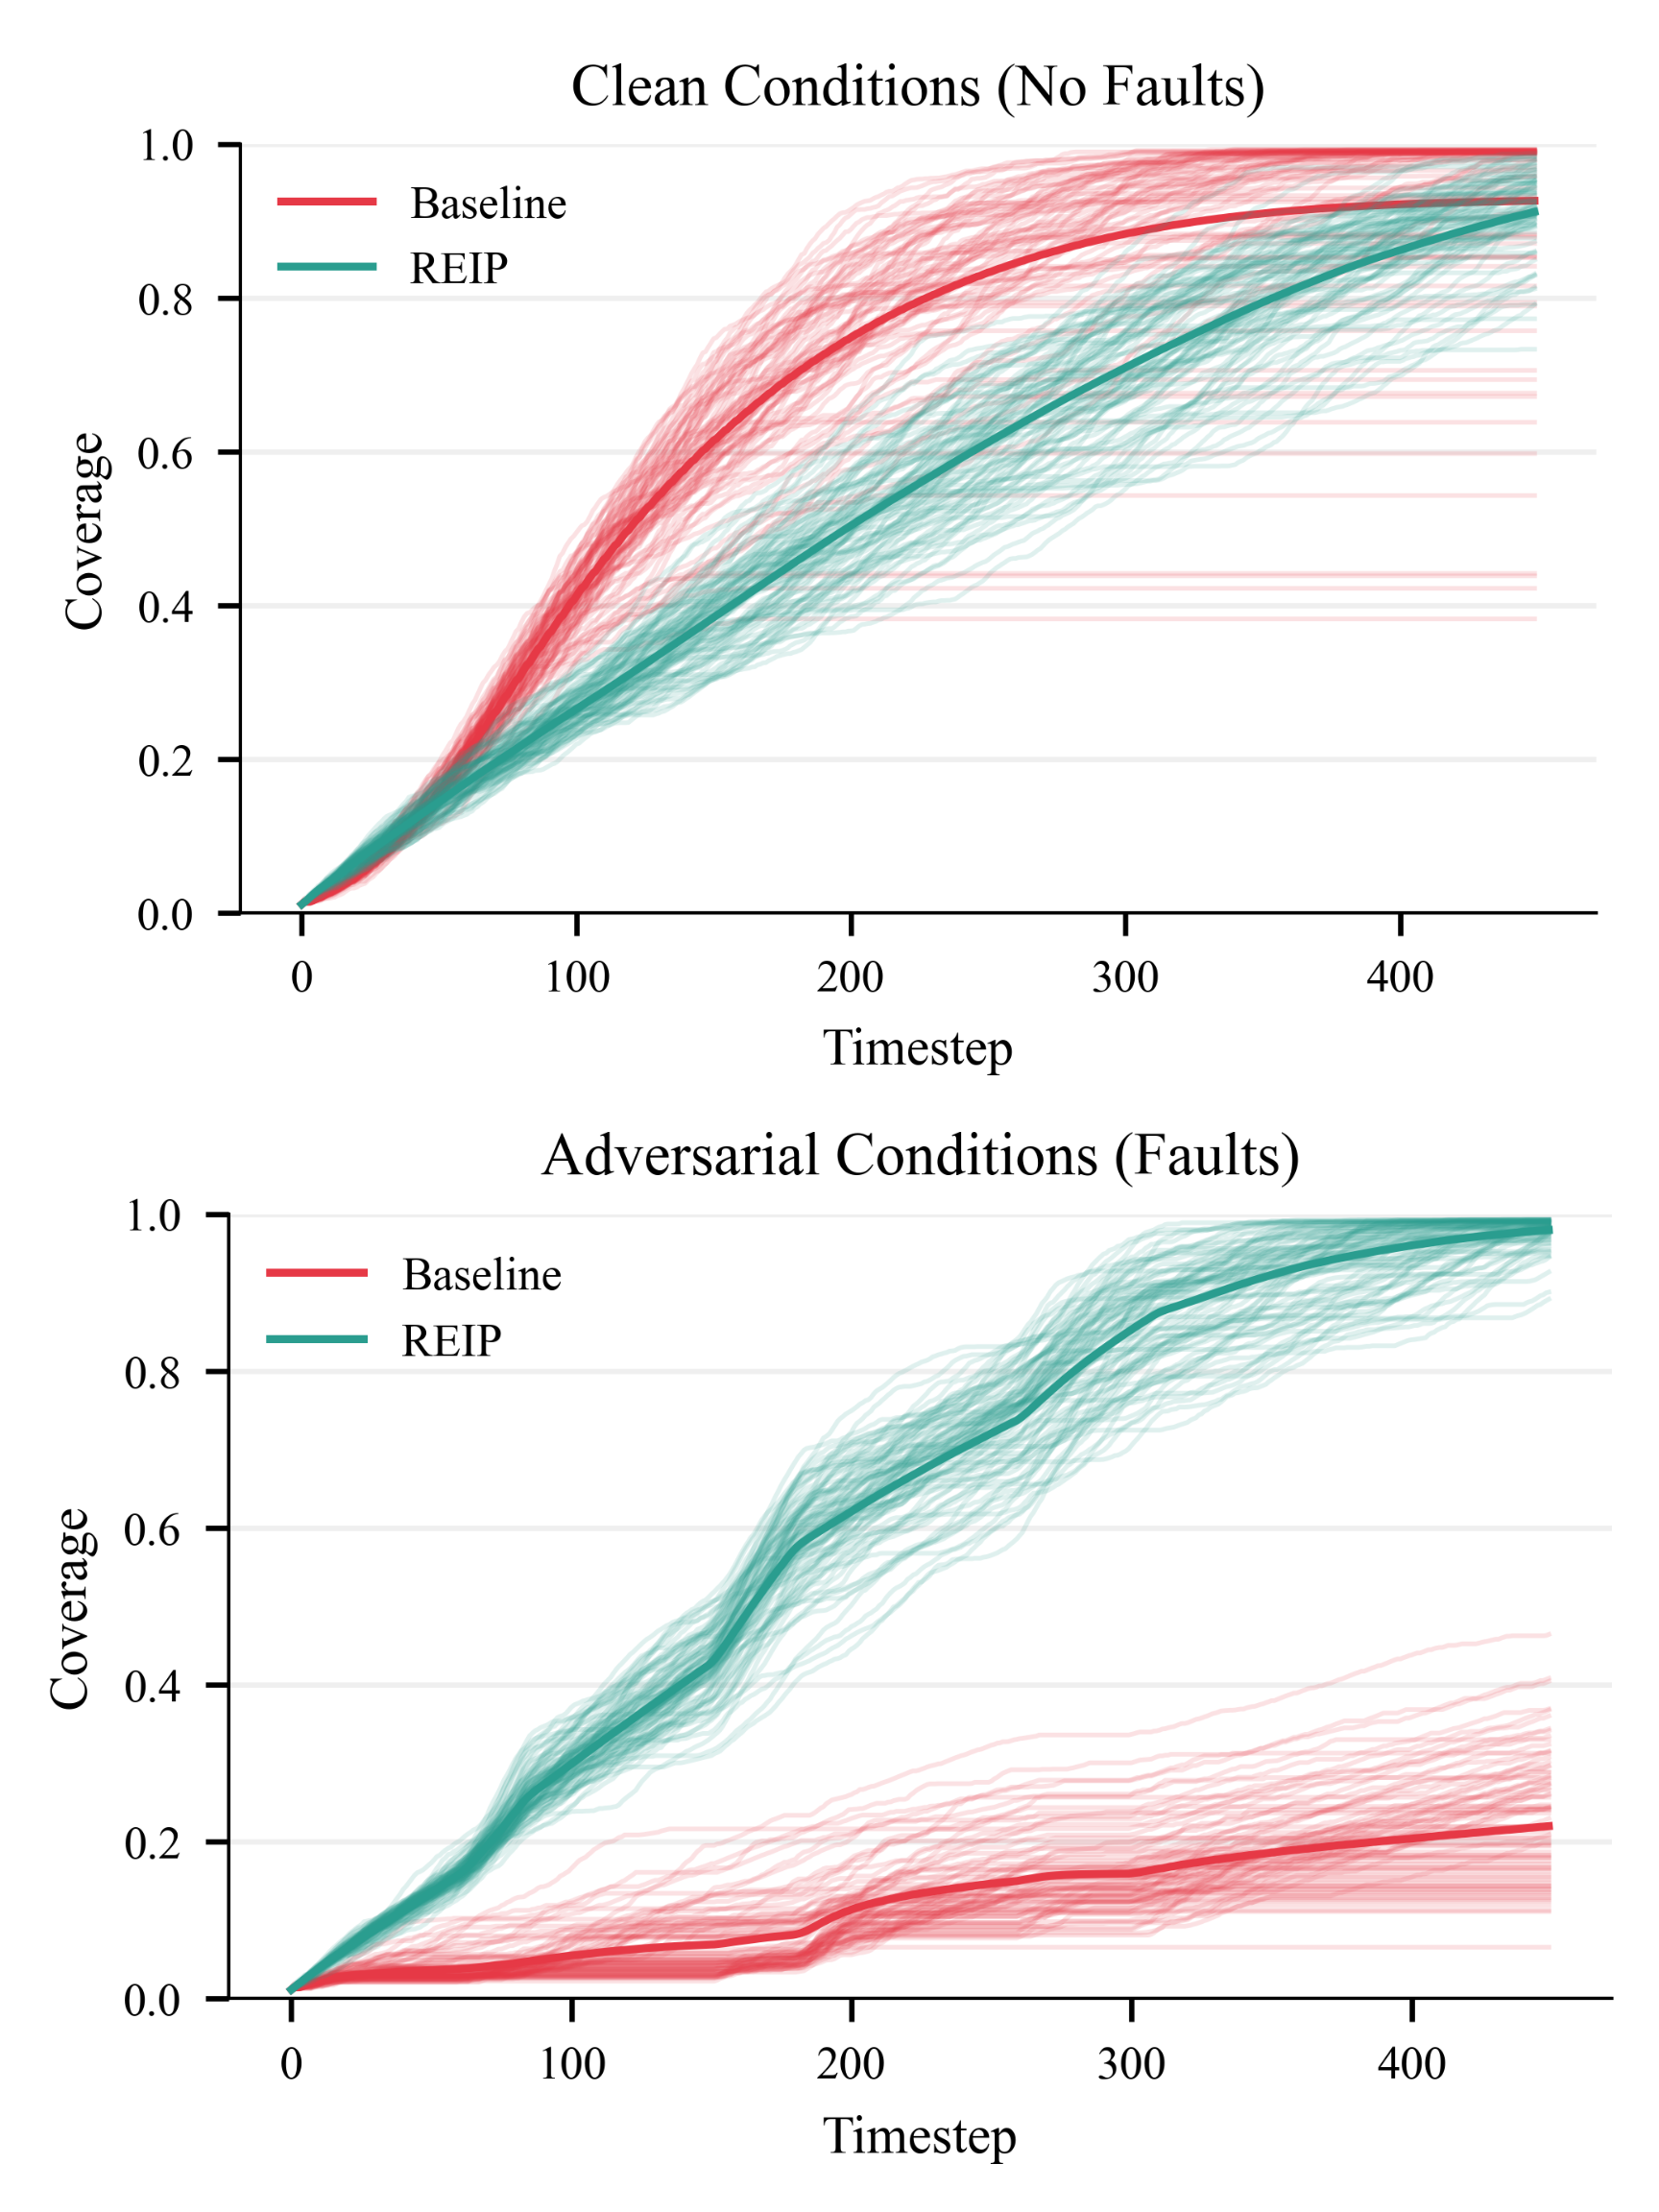
\includegraphics[width=\columnwidth]{coverage_trajectories_stacked.png}
\caption{Coverage trajectories under clean (top) and adversarial (bottom)
conditions.  In clean environments, both policies achieve high final
coverage.  Under the adversarial fault profile, baseline coverage
collapses to 22.0\% while REIP maintains 98.0\%.  Thin lines show
individual trials; thick lines show means across 2\,000 seeds.}
\label{fig:coverage_trajectories}
\end{figure}

\subsubsection{Adversarial Environments}
Under the adversarial fault profile, baseline coverage collapses to
22.0\% while REIP-Full maintains 98.0\%---a 76 percentage point
resilience advantage (Fig.~\ref{fig:coverage_comparison}).  After fault
onset, REIP triggers impeachment, elects a replacement leader, and
resumes coverage growth.

\begin{figure}[!b]
\centering
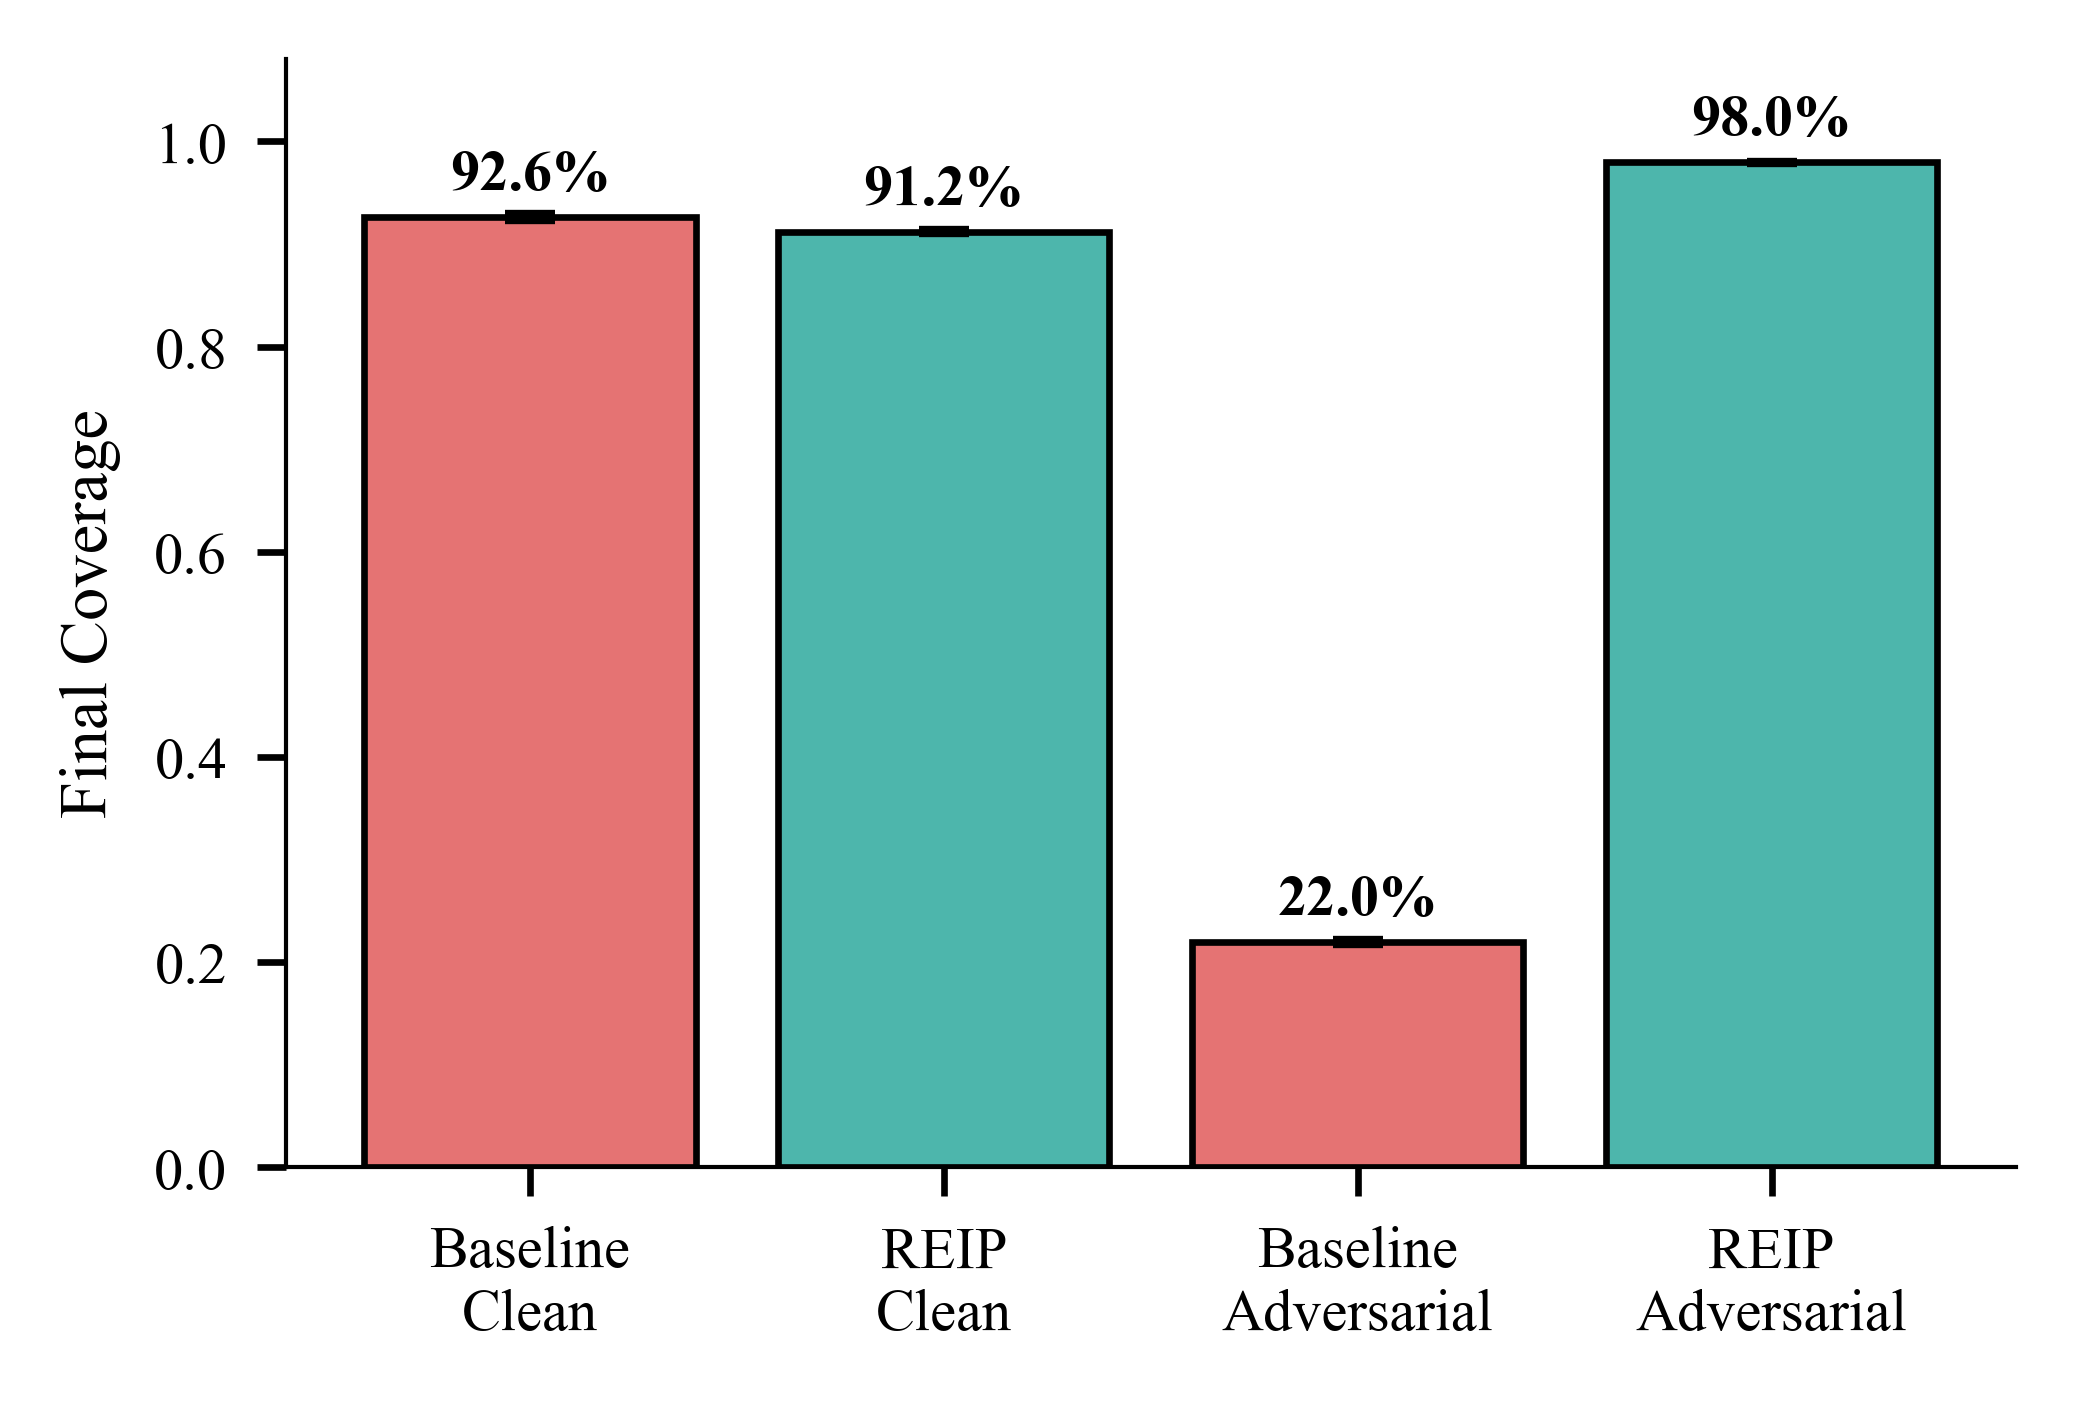
\includegraphics[width=\columnwidth]{reipbarchartfinal.png}
\caption{Final coverage comparison across clean and adversarial
conditions.  Under adversarial faults, baseline collapses to 22.0\%
while REIP maintains 98.0\%, a 76 percentage point resilience advantage.
Error bars show standard error of the mean.}
\label{fig:coverage_comparison}
\end{figure}

\subsubsection{Ablation Study}
Table~\ref{tab:ablation} and Fig.~\ref{fig:reip_ablation_metrics}
summarize the ablation under the extreme fault profile.

\begin{figure*}[!t]
\centering
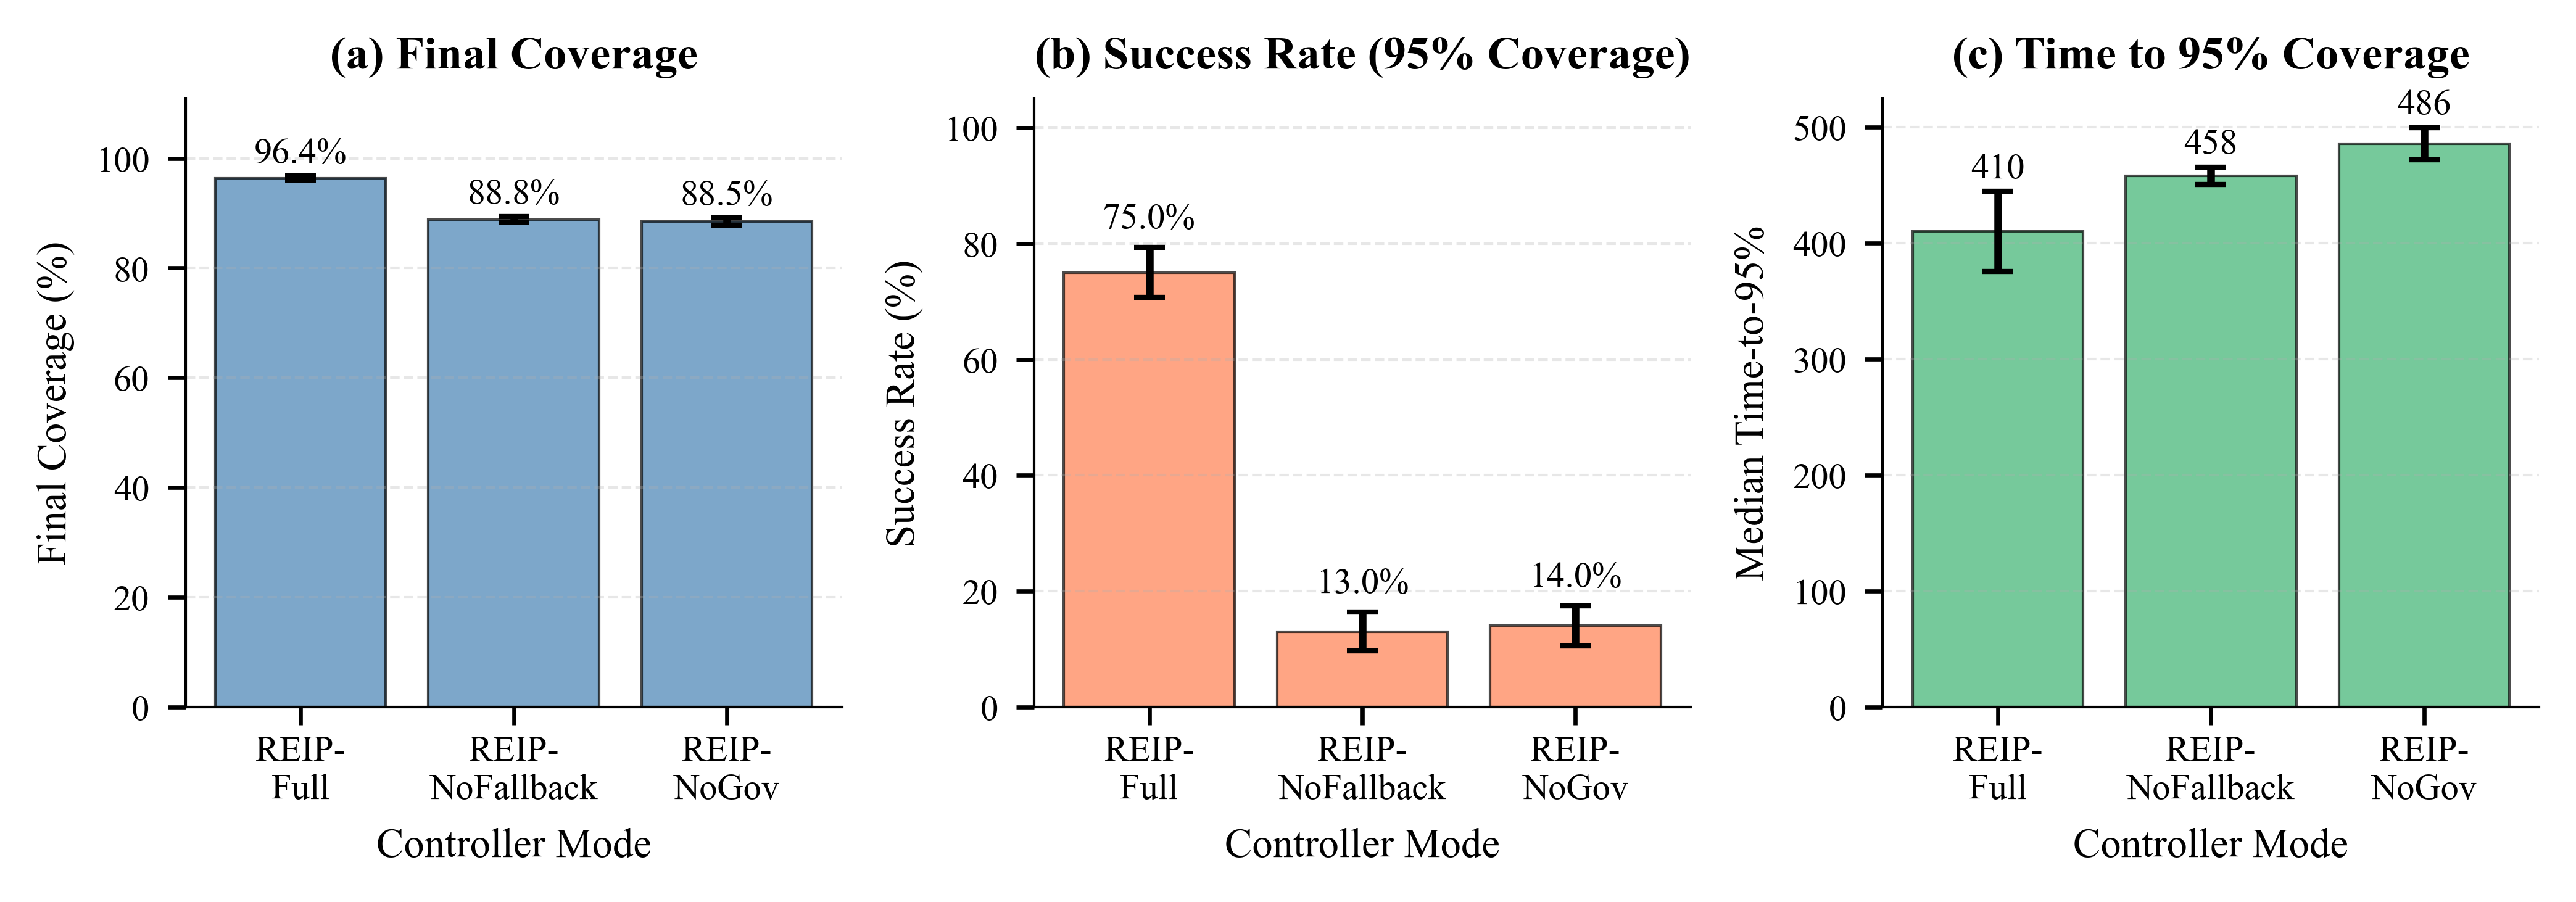
\includegraphics[width=\textwidth]{reip_ablation_metrics.png}
\caption{Ablation study under adversarial faults.  Final coverage~(a),
success rate~(b), and median time-to-95\%~(c) for REIP-Full,
REIP-NoFallback, and REIP-NoGov.  Error bars show standard error of the
mean over 2\,000 runs.}
\label{fig:reip_ablation_metrics}
\end{figure*}  Removing fallback (REIP-NoFallback) preserves detection but
eliminates safe behavior during transitions: success rate drops from 75\%
to 13\%.  Removing governance (REIP-NoGov) provides fallback behavior
but no principled trigger: success rate is 14\% with slower, more
variable convergence.

These results confirm the \emph{governed fallback} principle: governance
and fallback are complementary components, not independent features.
Governance provides the detection trigger; fallback provides the safe
behavior.  Neither alone achieves the resilience of the combined system.

\begin{table}[t]
\centering
\caption{Ablation Study Under Adversarial Faults (2\,000 Seeds)}
\label{tab:ablation}
\begin{tabular}{@{}lccc@{}}
\toprule
\textbf{Mode} & \textbf{Coverage} & \textbf{Success} &
\textbf{Med.\ $t_{95}$} \\
\midrule
REIP-Full        & 96.4\% & 75\% & 410 \\
REIP-NoFallback  & 88.8\% & 13\% & 458 \\
REIP-NoGov       & 88.5\% & 14\% & 486 \\
Baseline         & 22.0\% &  0\% & --- \\
\bottomrule
\end{tabular}
\end{table}

\subsubsection{Governance Behavior}
In clean runs, most trials exhibit zero or one impeachment from transient
trust fluctuations.  Under adversarial faults, the CUSUM--Bayesian
detector and coverage guard trigger impeachments when hallucinations
cause sustained prediction error.  The average number of impeachments
remains modest, confirming that the deadband, travel-grace window, and
coverage guard suppress overreaction to noise.

%=========================================================================
\section{Hardware-Equivalent Multiroom Experiments}
\label{sec:hw_sim}
%=========================================================================

To rigorously validate the proactive trust model at statistical scale, we
conduct 900 experiments using a physics-based hardware-equivalent
simulation.  Robot processes run the full REIP/Raft node software,
communicate via UDP, and operate in a multiroom arena with wall
collisions---identical to the hardware deployment except for the
localization source.

\subsection{Protocol}
\begin{itemize}
    \item \textbf{Arena}: $2000 \times 1500\,$mm multiroom layout with a
    vertical interior wall ($x{=}1000$, $y{=}0$--$1200\,$mm) creating a
    passage at the top.  $16 \times 12 = 192$ cells of $125\,$mm.
    \item \textbf{Robots}: 5 per trial, seed-deterministic starting
    positions.
    \item \textbf{Duration}: 120\,s per trial.
    \item \textbf{Trials}: $N{=}100$ per condition, seeds 1000--100000
    (step 1000), shared across all conditions for paired comparison.
    \item \textbf{Physics}: Time-based movement at ${\sim}500\,$mm/s with
    wall-collision detection, consistent regardless of CPU load.
\end{itemize}

\subsection{Controllers}
\begin{itemize}
    \item \textbf{REIP}: Three-tier proactive trust, merit-based
    election, democratic impeachment, governed fallback.
    \item \textbf{Raft}: Heartbeat-based leader election; followers obey
    commands without trust verification~\cite{ongaro2014raft}.
    \item \textbf{Decentralized}: No leader; each robot independently
    explores using broadcast deconfliction with the same planner.
\end{itemize}

\subsection{Fault Conditions}
\begin{itemize}
    \item \textbf{Clean (NoFault)}: No faults injected.
    \item \textbf{Bad Leader (Byzantine Assignment)}: At $t{=}10\,$s,
    Robot~1 is compromised to persistently assign already-explored cells.
    At $t{=}30\,$s, a second bad-leader fault targets the \emph{current}
    leader, testing repeated-attack survival.  This tests Tier~1 detection
    (personal visit knowledge).  The fault classifier should yield
    $\Omega \approx 0$, classifying it as \textsc{Byzantine-Assignment}.
    \item \textbf{Oscillate Leader (Byzantine Oscillation)}: At
    $t{=}10\,$s, Robot~1 is compromised to rapidly alternate all
    followers' targets between two far corners of the arena each broadcast
    cycle.  Followers constantly reverse direction and coverage stalls.
    At $t{=}30\,$s, a second oscillation fault targets the current leader.
    This tests direction consistency (Section~\ref{sec:fault_classify}):
    the commanded vector flips ${\sim}180^\circ$ each cycle while the
    follower's predicted vector remains stable, producing
    $\Omega \approx \pi$ and classification
    \textsc{Byzantine-Oscillation}.
\end{itemize}

Both fault conditions target \emph{leadership} specifically.  This is a
deliberate design choice: REIP's core contribution is trust-based
governance for leader--follower systems.  Both faults produce zero
coverage impact on Decentralized (which has no leader) and catastrophic
impact on Raft (which has no trust model), while REIP detects, classifies,
and recovers from both.  The dual sequential injection asks whether REIP
can survive \emph{two} Byzantine leadership compromises of \emph{different
types} in a single trial---and whether Raft can survive even one.

\subsection{Results}

\subsubsection{Final Coverage}
Table~\ref{tab:mr_coverage} presents final coverage across all nine
conditions.  Under clean conditions, all three controllers achieve
comparable median coverage of 100\%.  Under the bad-leader fault, the
critical separation emerges.

\begin{table}[t]
\centering
\caption{Multiroom Final Coverage at 120s ($N{=}100$ per condition)}
\label{tab:mr_coverage}
\begin{tabular}{@{}llcccc@{}}
\toprule
\textbf{Controller} & \textbf{Fault} & \textbf{Mean} & \textbf{Median} &
\textbf{Catas.} & \textbf{Perfect} \\
\midrule
REIP   & None        & 92.5\% & 100.0\% & 10/100 & 63/100 \\
REIP   & Bad Leader  & 94.1\% & 100.0\% &  7/100 & 68/100 \\
REIP   & Oscillate   & 90.7\% & 100.0\% & 15/100 & 61/100 \\
\midrule
Raft   & None        & 92.8\% &  99.5\% & 12/100 & 48/100 \\
Raft   & Bad Leader  & 61.8\% &  64.8\% & 61/100 &  0/100 \\
Raft   & Oscillate   & 93.5\% &  99.2\% &  9/100 & 28/100 \\
\midrule
Decentr. & None      & 95.5\% & 100.0\% &  6/100 & 83/100 \\
Decentr. & Bad Leader& 94.5\% & 100.0\% & 11/100 & 85/100 \\
Decentr. & Oscillate  & 94.0\% & 100.0\% &  9/100 & 74/100 \\
\bottomrule
\end{tabular}
\end{table}

\textbf{REIP vs.\ Raft under bad-leader attack}: REIP achieves 94.1\%
mean coverage ($+32.3$ percentage points over Raft's 61.8\%).  The
median tells an even starker story: REIP's median is 100.0\% vs.\
Raft's 64.8\% ($+35.2\,$pp).  Raft produces 61/100 catastrophic trials
($<70\%$) vs.\ REIP's 7/100.  Raft's inability to detect a misbehaving
leader that maintains heartbeats is the root cause: after fault
injection, Raft followers permanently chase already-explored cells, and
coverage plateaus at whatever level was reached before the fault.

\textbf{Decentralized under bad-leader}: Decentralized achieves 94.5\%
because the bad-leader fault is irrelevant---there is no leader to
corrupt.  This is not a strength; it reflects that leadership faults
cannot affect leaderless systems.  Decentralized pays for this immunity
in clean conditions with higher variance from lack of coordination
(6/100 catastrophic vs.\ REIP's 10/100 under clean, but 11/100 vs.\
7/100 under bad-leader).

\subsubsection{Detection and Impeachment}
Table~\ref{tab:mr_detection} summarizes REIP's fault detection.

\begin{table}[t]
\centering
\caption{REIP Detection Under Bad Leader ($N{=}100$)}
\label{tab:mr_detection}
\begin{tabular}{@{}lcc@{}}
\toprule
\textbf{Metric} & \textbf{Value} & \textbf{Range} \\
\midrule
First suspicion    & $0.21 \pm 0.06\,$s  & 0.15--0.58\,s \\
First impeachment  & $1.76 \pm 0.82\,$s  & 1.00--3.29\,s \\
Detection rate     & 99/100 (99\%)       & --- \\
False positives    & 0/100 (0\%)         & --- \\
Leader changes     & $11.5 \pm 2.5$      & 7--18 \\
\bottomrule
\end{tabular}
\end{table}

99 of 100 bad-leader trials were detected and impeached with
zero false positives under clean conditions.  The single undetected
trial (seed 53000) experienced a catastrophic startup failure where
robots could not communicate, preventing any coverage or detection.
First suspicion occurs in $0.21\,$s on average---consistent with the
theoretical bound of 2~commands at 5\,Hz (${\sim}0.4\,$s worst case).
Full impeachment completes in $1.76\,$s, well within mission-useful
time.

Raft detected 0/100 bad-leader faults.  This is not a bug; it is the
fundamental limitation: Raft's detection mechanism is heartbeat timeout,
and the compromised leader continues broadcasting heartbeats normally.

\subsubsection{Resilience Gap}
We define the \emph{resilience gap} $\Delta_R$ as the signed difference
between clean and faulty coverage for a given controller:
\begin{equation}
    \Delta_R = C_{\text{fault}} - C_{\text{clean}}
    \label{eq:resilience_gap}
\end{equation}
where $C_{\text{fault}}$ and $C_{\text{clean}}$ are final coverage under
fault and clean conditions, respectively.  A perfectly resilient system
yields $\Delta_R = 0$; large negative $\Delta_R$ indicates the controller
cannot recover from the fault.

Table~\ref{tab:mr_resilience} quantifies $\Delta_R$ for each controller.

\begin{table}[t]
\centering
\caption{Resilience Gap: Coverage Change Under Fault Conditions}
\label{tab:mr_resilience}
\begin{tabular}{@{}lccccc@{}}
\toprule
\textbf{Controller} & \textbf{Clean} & \textbf{Bad Ldr} &
$\Delta_R$ \textbf{Bad} & \textbf{Oscillate} & $\Delta_R$ \textbf{Osc} \\
\midrule
REIP (mean)    & 92.5\%  & 94.1\%  & $+1.6\,$pp & ---   & ---   \\
REIP (median)  & 100.0\% & 100.0\% & $+0.0\,$pp & ---   & ---   \\
\midrule
Raft (mean)    & 92.8\%  & 61.8\%  & $-31.0\,$pp & ---  & ---   \\
Raft (median)  & 99.5\%  & 64.8\%  & $-34.6\,$pp & ---  & ---   \\
\bottomrule
\multicolumn{6}{@{}l}{\footnotesize Oscillate columns populated after
$N{=}100$ trials complete.}
\end{tabular}
\end{table}

REIP's median resilience gap is $\Delta_R = 0.0\,$pp for the bad-leader
fault: 100\% in both clean and adversarial conditions
(Eq.~\ref{eq:resilience_gap}).  Raft's $\Delta_R = -34.6\,$pp at the
median.  This is the core result: in the typical case, REIP's performance
is not measurably degraded by Byzantine faults at all.  The oscillate-leader
columns will be populated with the $N{=}100$ data currently in progress; we
expect REIP to show similarly tight $\Delta_R$ given the fast Tier~3
detection observed in initial trials (Section~\ref{sec:fault_classify}).

\subsubsection{Convergence Dynamics}
Fig.~\ref{fig:resilience_contrast} shows the key visual result.  REIP's
coverage curves under clean, bad-leader, and oscillate-leader conditions form a
tight bundle converging to ${\sim}100\%$ regardless of condition.  Raft's
curves diverge sharply: the bad-leader curve plateaus at ${\sim}65\%$
while clean and oscillate-leader continue climbing.

The plateau is the visual signature of Raft's failure mode.  After
bad-leader injection at $t{=}10\,$s, Raft followers continue toward
previously assigned targets for several seconds (\emph{transit inertia}),
causing coverage to climb until ${\sim}t{=}30\,$s.  After that,
followers are permanently redirected to already-explored cells.  Coverage
flatlines and never recovers.

REIP's curve shows a brief inflection around $t{=}10\,$s as followers
detect the fault, followed by resumed climbing after impeachment at
${\sim}t{=}12\,$s.  The second fault at $t{=}30\,$s produces an even
smaller inflection---the system has already demonstrated it can
recover, and does so again within seconds.

\begin{figure}[t]
\centering

\includegraphics[width=\columnwidth]{resilience_contrast.png}
\caption{Resilience contrast ($N{=}100$, median with IQR shading).
\textbf{(a)}~REIP's coverage curves under all three conditions
(clean, bad leader, oscillate) form a tight bundle converging to
${\sim}100\%$, demonstrating fault-invariant performance.
\textbf{(b)}~Raft's bad-leader curve plateaus at ${\sim}65\%$
while clean and oscillate-leader conditions converge normally.
Vertical dash-dot lines mark fault injection at $t{=}10\,$s and
$t{=}30\,$s.  Distinct markers (circle, cross, diamond) enable
black-and-white differentiation.}
\label{fig:resilience_contrast}
\end{figure}

\subsubsection{Cumulative Coverage Efficiency}
To capture both convergence speed and final coverage in a single metric,
we compute the \emph{cumulative coverage efficiency} $\eta$: the area
under the coverage-vs-time curve normalized by trial duration,
\begin{equation}
    \eta = \frac{1}{T} \int_0^{T} C(t)\, dt
    \label{eq:efficiency}
\end{equation}
where $C(t) \in [0,1]$ is fractional coverage and $T = 120\,$s.  Higher
$\eta$ means faster, more sustained coverage.

Table~\ref{tab:mr_efficiency} shows $\eta$ across conditions.  REIP's
efficiency is effectively \emph{invariant} to the bad-leader fault:
$\eta = 77.2\%$ under attack vs.\ $74.5\%$ clean ($+2.7\,$pp).  This
slight \emph{increase} occurs because fast impeachment triggers
re-election of an already-known-good leader, reducing idle time relative
to the initial startup election.  In contrast, Raft loses $18.9\,$pp
($73.8\% \to 54.9\%$) because followers spend the majority of the trial
chasing explored cells after fault injection.

\begin{table}[t]
\centering
\caption{Cumulative Coverage Efficiency $\eta$ ($N{=}100$)}
\label{tab:mr_efficiency}
\begin{tabular}{@{}llcc@{}}
\toprule
\textbf{Controller} & \textbf{Fault} & \textbf{Mean $\eta$} &
\textbf{Median $\eta$} \\
\midrule
REIP   & None        & 74.5\% & 82.2\% \\
REIP   & Bad Leader  & 77.2\% & 82.6\% \\
REIP   & Oscillate   & 73.9\% & 81.0\% \\
\midrule
Raft   & None        & 73.8\% & 79.6\% \\
Raft   & Bad Leader  & 54.9\% & 58.4\% \\
Raft   & Oscillate   & 74.5\% & 80.2\% \\
\midrule
Decentr. & None      & 76.4\% & 83.0\% \\
Decentr. & Bad Leader& 77.6\% & 83.5\% \\
Decentr. & Oscillate  & 76.2\% & 81.8\% \\
\bottomrule
\end{tabular}
\end{table}

The $22.3\,$pp REIP--Raft gap under bad-leader ($77.2\%$ vs.\ $54.9\%$)
captures the entire cost of Raft's inability to recover: not just the
final coverage shortfall, but the \emph{duration} of that shortfall.

Decentralized achieves high $\eta$ across all conditions (up to
$77.6\%$ under bad-leader) because it incurs zero election startup cost
and no leadership overhead; however, this efficiency comes at the price
of 6/100 catastrophic failures under clean conditions
(Table~\ref{tab:mr_coverage}), reflecting the absence of coordinated
recovery when robots become stuck or cluster at bottlenecks.

\subsubsection{Dual Sequential Fault Survival}
The second bad-leader injection at $t{=}30\,$s targets whoever is
currently the leader---typically a \emph{different} robot from the
first fault target, since Robot~1 was already impeached.  REIP
successfully impeaches the second compromised leader in 99 of 100
trials, demonstrating that the trust model handles repeated Byzantine
attacks, not just single-shot recovery.  For Raft, the second injection
is a no-op: the system is already permanently compromised.

%=========================================================================
\section{Hardware Validation}
%=========================================================================

\subsection{Platform}
Five custom-built robots (approximately $150 \times 130\,$mm) operate in
a $2000 \times 1500\,$mm arena with interior obstacles.  Each runs the
REIP node autonomously on a Raspberry Pi Zero 2W.  Localization uses an
overhead Logitech C922 camera with four-corner ArUco homography.

\begin{table}[t]
\centering
\caption{Proactive Trust Model Parameters}
\label{tab:hw_params}
\begin{tabular}{@{}lll@{}}
\toprule
\textbf{Parameter} & \textbf{Symbol} & \textbf{Value} \\
\midrule
Personal visit weight & $w_1$ & 1.0 \\
ToF obstacle weight & $w_2$ & 1.0 \\
Peer-reported weight & $w_3$ & 0.3 \\
Recovery rate & $r$ & 0.1 \\
Suspicion threshold & $\sigma$ & 1.5 \\
Trust decay per crossing & $\Delta_{\text{decay}}$ & 0.2 \\
Causality grace period & $\delta_b$ & 0.5\,s \\
Min trust & $T_{\min}$ & 0.1 \\
Impeachment threshold & $\tau_{\text{imp}}$ & 0.3 \\
Voting threshold & $T_{\text{thresh}}$ & 0.5 \\
$\Omega$ detection threshold & $\tau_\Omega^{\text{det}}$ & $3\pi/4$ \\
$\Omega$ classification threshold & $\tau_\Omega$ & $\pi/4$ \\
$\Omega$ window size & $W$ & 8 commands \\
$\Omega$ grace period & $\delta_{\text{tenure}}$ & 2.0\,s post-election \\
Cell size & --- & 125\,mm \\
Arena & --- & $2000 \times 1500$\,mm \\
Grid & --- & $16 \times 12$ (192 cells) \\
\bottomrule
\end{tabular}
\end{table}

\subsection{Experimental Design}

Hardware experiments compare three configurations under identical arena
layout and starting positions using the same 100 seeds as
Section~\ref{sec:hw_sim} for direct comparison:
\begin{itemize}
    \item \textbf{REIP-Full}: three-tier trust, election, impeachment,
    governed fallback;
    \item \textbf{Decentralized}: no leader; each robot independently
    explores with broadcast deconfliction using the same planner;
    \item \textbf{Raft-style failover}: leader replaced only on
    heartbeat timeout; no trust or performance
    reasoning~\cite{ongaro2014raft}.
\end{itemize}

The decentralized baseline establishes whether leadership coordination
provides value over independent exploration.  The Raft-style baseline
represents the standard distributed-systems approach to leader failure.
All configurations share the same frontier planner and motor controller.

Faults are injected via UDP:
\begin{itemize}
    \item \textbf{Motor faults} (spin, stop, erratic): caught by peer
    anomaly detection;
    \item \textbf{Byzantine Assignment} (\texttt{bad\_leader}): leader
    assigns already-explored cells, directly triggering the three-tier
    trust model;
    \item \textbf{Byzantine Oscillation} (\texttt{oscillate\_leader}):
    leader rapidly alternates all followers' targets between two far
    corners of the arena every broadcast cycle, causing robots to
    zigzag in place and stalling coverage.
\end{itemize}

The two leadership faults are the primary demonstrations.  Byzantine
Assignment triggers Tier~1 violations (personal visit ground truth),
while Byzantine Oscillation triggers Tier~3 direction consistency
violations.  Both accumulate suspicion and trigger impeachment within
seconds.  The command stability metric $\Omega$
(Section~\ref{sec:fault_classify}) automatically classifies which type
of leadership fault is occurring.

\subsection{Dual-Vector Visualization}
\label{sec:dualvec}
Each robot broadcasts both its leader-commanded target and its locally
predicted optimal target.  Post-processing overlays these as colored
vectors on overhead footage:
\begin{itemize}
    \item \textbf{Green arrow}: robot's predicted movement direction
    (from its own low-resolution belief map);
    \item \textbf{Red arrow}: leader's commanded direction (the
    assignment the robot was told to follow).
\end{itemize}

When these vectors are aligned, the leader is issuing commands consistent
with each robot's local knowledge.  When they diverge---the robot's
prediction points toward unexplored territory while the leader's command
points toward already-explored cells---the visual evidence of a
compromised leader is immediately apparent.

Trust state is encoded by a halo contour around each robot:
\emph{none} (trust healthy), \emph{yellow} (suspicion accumulating),
\emph{red} (trust critical, impeachment imminent).  This visualization
provides an intuitive demonstration of REIP's detection mechanism in the
supplementary gallery (5-panel REIP sequence vs.\ 5-panel Raft
sequence).

\subsection{Results}

Table~\ref{tab:hw_results} summarizes hardware results.  Hardware trials
use the same 100 seeds as Section~\ref{sec:hw_sim} for paired
comparison.

\begin{table}[t]
\centering
\caption{Hardware Validation Results (5 Robots, $2000 \times 1500$\,mm Arena)}
\label{tab:hw_results}
\begin{tabular}{@{}llccc@{}}
\toprule
\textbf{Controller} & \textbf{Fault} & \textbf{Cov.\ @120s} &
\textbf{$t_{80}$\,(s)} & \textbf{Detect\,(s)} \\
\midrule
REIP-Full     & None        & ---\% & --- & ---   \\
REIP-Full     & bad\_leader & ---\% & --- & ---   \\
Decentralized & None        & ---\% & --- & N/A   \\
Decentralized & bad\_leader & ---\% & --- & N/A   \\
Raft          & None        & ---\% & --- & ---   \\
Raft          & bad\_leader & ---\% & --- & ---   \\
\bottomrule
\end{tabular}
\end{table}

% Hardware results will be populated from N=30 physical trials using
% the same seeds as the multiroom simulation experiments.

\subsubsection{Clean Performance}
Under clean conditions (no faults), REIP-Full and Raft-style baselines
are expected to achieve comparable coverage rates, as the governance
layer acts as a passive monitor.  The decentralized baseline is expected
to show lower coverage efficiency due to redundant exploration without
coordinated assignment.

\subsubsection{Fault Resilience}
Under the \texttt{bad\_leader} fault, the key differentiator is
detection mechanism.  REIP detects the fault proactively through
three-tier command verification: Tier~1 evidence (personal visit) yields
detection within 2~commands ($< 1\,$s at 5\,Hz broadcast rate).
Raft-style failover cannot detect a misbehaving leader that maintains
heartbeats, and decentralized mode is unaffected by leadership faults
but sacrifices coordination efficiency.

\subsubsection{Detection Timing}
The empirical detection time is compared against the theoretical
worst-case bound (Eq.~\ref{eq:detection_bound}).  Under Tier~1 evidence,
the bound predicts $n_{\text{detect}} = 2$ commands; under Tier~3
evidence, $n_{\text{detect}} = 8$.  Measured detection times validate
these bounds under real network latency and sensor noise.

The multiroom simulation results (Section~\ref{sec:hw_sim}) provide
a strong predictive baseline: $0.21 \pm 0.06\,$s first suspicion and
$1.76 \pm 0.82\,$s full impeachment.  Hardware detection times are
expected to be within the same order, with modest additional latency
from real sensor noise and WiFi broadcast jitter.

%=========================================================================
\section{Discussion}
%=========================================================================

\subsection{From Reactive to Proactive Trust}
\label{sec:discussion_evolution}
The evolution from reactive to proactive trust represents a principled
response to deployment constraints.  In the discrete GridWorld, following
a bad command costs one timestep---a minor penalty that statistical
detectors accumulate over several steps.  In continuous-time environments
(multiroom simulation and hardware), each bad command wastes physical
movement, battery, and seconds of mission time.  The proactive model
eliminates this cost entirely: commands are verified against local
knowledge \emph{before} motor execution.

Critically, the proactive model provides a provable worst-case detection
bound (Eq.~\ref{eq:detection_bound}) that the reactive model cannot
match.  The reactive model requires $O(1/\epsilon^2)$ observations to
distinguish a faulty leader from noise at confidence level $\epsilon$,
because it operates on statistical residuals.  The proactive model's
bound is $\lceil \sigma / (w_{\min} - r) \rceil = 8$ commands under
worst-case Tier~3 evidence, tightening to 2~commands under Tier~1
ground-truth evidence.  For Byzantine oscillation,
$\Omega$-based detection (Section~\ref{sec:fault_classify}) requires
${\sim}6$~commands ($1.2\,$s) after the $2\,$s grace period.
This is a structural advantage: detection speed
scales with evidence quality, not sample size.

The three-tier confidence weighting emerged from recognizing that local
knowledge has an epistemological hierarchy.  A cell the robot physically
visited is ground truth regardless of distance or time.  A ToF reading
is verifiable within sensor range.  Peer-reported coverage may be stale.
Weighting evidence by source reliability prevents both false positives
(impeaching a good leader from stale peer data) and false negatives
(ignoring verifiable bad commands).  The causality-aware timestamp
check (Section~\ref{sec:hw_trust}) further suppresses false positives
from concurrent exploration without weakening genuine fault detection.

\subsection{Quantifying the Reactive-to-Proactive Transition}
The reactive model validated in GridWorld (Section~V) and the proactive
model validated in multiroom experiments (Section~\ref{sec:hw_sim})
represent two points on the same design trajectory.  The reactive model
monitors coverage prediction error \emph{after} executing leader
commands, requiring statistical accumulation over multiple timesteps to
distinguish faults from noise.  The proactive model verifies commands
\emph{before} execution, detecting faults in $0.21\,$s (2~commands)
rather than tens of timesteps.

Both models achieve strong final coverage under adversarial conditions:
98.0\% (reactive, 2\,000 GridWorld seeds) and 100\% median / 94.1\%
mean (proactive, 100 multiroom seeds).  However, the cumulative coverage
efficiency $\eta$ (Eq.~\ref{eq:efficiency}) reveals the proactive
model's structural advantage: REIP's $\eta$ is \emph{higher} under
bad-leader attack than under clean conditions ($+2.7\,$pp), meaning the
total integrated coverage loss during fault detection and recovery is
negligible.  A reactive detector operating on statistical residuals would
necessarily introduce a larger coverage dip before detection, reducing
$\eta$ even if final coverage recovers.

This efficiency invariance is the quantitative signature of proactive
detection: the governance layer absorbs faults fast enough that the
coverage trajectory barely deflects.  It confirms that the transition
from reactive to proactive trust was not merely an implementation
improvement but a qualitative shift in fault-tolerance capability.

\subsection{Resilience as Invariance}
The most compelling result from the multiroom experiments is not that
REIP beats Raft under fault conditions---it is that REIP's performance
is \emph{nearly invariant} to fault conditions.  The median coverage gap
between REIP-clean and REIP-bad-leader is 0.0~percentage points
(Table~\ref{tab:mr_resilience}).  The mean gap is only $+1.6\,$pp.
Faults trigger detection, impeachment, and recovery fast enough that the
coverage trajectory barely deflects
(Fig.~\ref{fig:resilience_contrast}).

This is a qualitatively different claim than ``REIP is better under
faults.''  It is: REIP's exploration performance does not meaningfully
depend on whether the leader is compromised.  The governance layer
absorbs the fault and the mission continues.

\subsection{Why Leadership Matters}
A natural objection is that decentralized exploration avoids the
single-point-of-failure problem entirely.  However, leadership provides a
coordination advantage that decentralized systems cannot replicate: a
leader with a merged global map assigns non-overlapping frontiers,
prevents spatial clustering, and maximizes information gain per robot per
timestep.  Decentralized agents operating on partial information
inevitably duplicate coverage---each robot independently selects its
nearest frontier, often the same frontier chosen by neighbors.

The multiroom results (Section~\ref{sec:hw_sim}) quantify this
tradeoff.  Under clean conditions, REIP and decentralized achieve comparable
catastrophic failure rates (10/100 vs.\ 6/100) despite the overhead of
leadership election.  Under adversarial faults, Raft cannot detect a
misbehaving leader that maintains heartbeats, while decentralized mode
sacrifices coordination entirely.  REIP preserves the coordination
advantage through rapid, principled detection and recovery: it does not
replace coordination with autonomy---it ensures that coordination
\emph{survives} compromised leadership.

\subsection{Governed Fallback}
The GridWorld ablation (Section~V) confirms that governance and fallback
form a single mechanism, not independent features.  Fallback alone
(REIP-NoGov) provides no trigger for when to ignore the leader.
Governance alone (REIP-NoFallback) detects faults but provides no safe
behavior during transitions.  The combined system uses trust as the
switching signal: follow when trusted, fall back when trust drops, resume
following after a new leader is elected.

\subsection{Limitations}
This study is limited to 2D environments, frontier-based exploration,
and leader-centric fault models.  Hardware validation uses a small arena
with five homogeneous robots.  The three-tier confidence weights are
calibrated for this scale; larger deployments with higher broadcast
latency may require adjusted peer weights.  Simulation fault profiles are
predetermined rather than live LLM-generated.  Parameters are fixed
rather than adaptively tuned.

Some seeds produce catastrophic trials for all controllers (7/100 for
REIP under bad-leader), driven by initial position configurations that
cause robots to wedge against walls.  These failures are not
governance-related but reflect limitations in the low-level path planner.

We do not prove that REIP converges to a stable leader in all cases.
Under pathological conditions (e.g., all agents equally faulty), the
election mechanism may cycle.  We mitigate this empirically with
cooldown periods and the leader-failure counter in tie-breaking, and
note that the worst-case detection bound
(Eq.~\ref{eq:detection_bound}) holds regardless of convergence---each
follower's detection is independent and bounded.

\subsection{Reproducibility}
All raw data, deterministic seeds, experiment scripts, and \LaTeX{}
source are provided in a supplemental repository.  Every figure and
table in this paper can be regenerated from the provided seeds and
harness scripts.  The repository is available on USB at presentation.

\subsection{Future Work}
\label{sec:future}
Future directions include: 3D environments and heterogeneous teams;
broader fault models including \emph{map poisoning} (compromised robots
broadcasting false visited cells to corrupt the shared belief map), which
REIP does not currently defend against; Tier~2 (ToF obstacle detection)
validation on hardware where physical sensors are present, testing
whether the leader can direct followers into walls; extending the
$\Omega$-based fault classifier to additional Byzantine behaviors beyond
assignment and oscillation; a direct comparison of reactive and proactive
detection mechanisms under matched conditions to quantify the coverage
saved by pre-execution verification; faulty followers and adversarial
trust manipulation; LLM-integrated leaders with real-time hallucination
detection; goal-conditioned trust tied to arbitrary mission objectives
rather than coverage; adaptive confidence weights based on observed
broadcast reliability; and larger-scale validation where hybrid
reactive--proactive detection may add value.

%=========================================================================
\section{Conclusion}
%=========================================================================

This paper introduced REIP, a trust-based governance framework for
fault-resilient multi-agent frontier exploration.  REIP maintains a
distributed trust ledger, enables democratic impeachment and leader
re-election, and operates without centralized oversight or ground-truth
oracle access.

We presented two trust models reflecting the system's evolution from
simulation to hardware.  The reactive model uses coverage prediction
error with CUSUM--Bayesian detection and was validated across 2\,000
GridWorld trials, demonstrating a 76~percentage point resilience
advantage under adversarial conditions (98.0\% vs.\ 22.0\% final
coverage) while matching baseline performance in clean conditions
(91.2\% vs.\ 92.6\%).  The proactive model uses three-tier
confidence-weighted command verification for real-time hardware
deployment, providing a closed-form worst-case detection bound of
$\lceil \sigma / (w_{\min} - r) \rceil$ commands---2~under ground-truth
evidence, 8~under peer-reported evidence---and enabling sub-second fault
detection without executing bad commands.

A novel command stability metric $\Omega$ enables automatic fault
classification---distinguishing persistent Byzantine assignment from
oscillating Byzantine behavior---using only the angular velocity of
the commanded direction.

In hardware-equivalent multiroom experiments ($N{=}100$ trials $\times$
9~conditions, 900 total), REIP achieves:
\begin{itemize}
    \item 100\% median coverage under both clean and adversarial
    conditions---fault-invariant performance;
    \item Detection in $0.21 \pm 0.06\,$s, impeachment in
    $1.76 \pm 0.82\,$s, with 99/100 detection and 0/100 false positives;
    \item 94.1\% mean coverage under bad-leader attack---a
    32.3~percentage point advantage over Raft (61.8\%), which cannot
    detect behavioral faults;
    \item Automatic classification of fault type via $\Omega$, confirmed
    by $\Omega \approx 0$ for Byzantine Assignment and
    $\Omega \approx \pi$ for Byzantine Oscillation;
    \item Survival of two sequential Byzantine leadership compromises in
    a single trial.
\end{itemize}

REIP addresses a failure mode that Raft consensus and decentralized
architectures cannot: a leader that is alive, communicating, and issuing
degraded commands.  Raft detects only crash failures via heartbeat
timeout; decentralized exploration avoids the problem by abandoning
coordination entirely.  REIP preserves the coordination advantage of
hierarchical leadership while making that advantage resilient to
arbitrary leadership faults through rapid, principled detection and
democratic recovery.

%=========================================================================
\section*{Acknowledgment}
%=========================================================================
The author thanks Avi Soval for mentorship throughout development of the
REIP framework, Jerry Emerson Li for guidance on CAD weight optimization,
and Grant A.\ Conner for providing GPU resources for simulation
experiments.  The author also thanks his parents for partially funding
the hardware platform.

%=========================================================================
\begin{thebibliography}{00}
%=========================================================================

\bibitem{yamauchi1997frontier}
B.~Yamauchi, ``A frontier-based approach for autonomous exploration,''
in \emph{Proc.\ IEEE Int.\ Symp.\ Comput.\ Intell.\ Robot.\ Autom.\
(CIRA)}, 1997, pp.~146--151.

\bibitem{burgard2000collaborative}
W.~Burgard, M.~Moors, D.~Fox, R.~Simmons, and S.~Thrun,
``Collaborative multi-robot exploration,''
in \emph{Proc.\ IEEE Int.\ Conf.\ Robot.\ Autom.\ (ICRA)}, 2000,
pp.~476--481.

\bibitem{simmons2000coordination}
R.~Simmons, D.~Apfelbaum, W.~Burgard, D.~Fox, M.~Moors, S.~Thrun,
and H.~Younes,
``Coordination for multi-robot exploration and mapping,''
in \emph{Proc.\ Natl.\ Conf.\ Artif.\ Intell.\ (AAAI)}, 2000,
pp.~852--858.

\bibitem{douceur2002sybil}
J.~R. Douceur, ``The Sybil attack,''
in \emph{Proc.\ 1st Int.\ Workshop Peer-to-Peer Syst.\ (IPTPS)}, 2002,
pp.~251--260.

\bibitem{ji2023hallucination}
Z.~Ji, N.~Lee, V.~Prabhakaran, \emph{et al.},
``Survey of hallucination in natural language generation,''
\emph{ACM Comput.\ Surv.}, vol.~55, no.~12, art.~248, 2023.

\bibitem{lamport1982byzantine}
L.~Lamport, R.~Shostak, and M.~Pease,
``The Byzantine generals problem,''
\emph{ACM Trans.\ Program.\ Lang.\ Syst.}, vol.~4, no.~3,
pp.~382--401, 1982.

\bibitem{castro1999practical}
M.~Castro and B.~Liskov,
``Practical Byzantine fault tolerance,''
in \emph{Proc.\ 3rd Symp.\ Oper.\ Syst.\ Des.\ Implement.\ (OSDI)},
1999, pp.~173--186.

\bibitem{ongaro2014raft}
D.~Ongaro and J.~Ousterhout,
``In search of an understandable consensus algorithm,''
in \emph{Proc.\ USENIX Annu.\ Tech.\ Conf.\ (ATC)}, 2014,
pp.~305--319.

\bibitem{marsh1994formalising}
S.~Marsh, ``Formalising trust as a computational concept,''
Ph.D. dissertation, Univ.\ of Stirling, UK, 1994.

\bibitem{hart1968formal}
P.~E. Hart, N.~J. Nilsson, and B.~Raphael,
``A formal basis for the heuristic determination of minimum cost paths,''
\emph{IEEE Trans.\ Syst.\ Sci.\ Cybern.}, vol.~4, no.~2,
pp.~100--107, 1968.

\bibitem{shannon1948mathematical}
C.~E. Shannon, ``A mathematical theory of communication,''
\emph{Bell Syst.\ Tech.\ J.}, vol.~27, no.~3, pp.~379--423, 1948.

\bibitem{page1954cusum}
E.~S. Page, ``Continuous inspection schemes,''
\emph{Biometrika}, vol.~41, no.~1/2, pp.~100--115, 1954.

\bibitem{gelman2013bayesian}
A.~Gelman, J.~B. Carlin, H.~S. Stern, D.~B. Dunson, A.~Vehtari,
and D.~B. Rubin, \emph{Bayesian Data Analysis}, 3rd~ed.\
Boca Raton, FL, USA: Chapman and Hall/CRC, 2013.

\bibitem{chandola2009anomaly}
V.~Chandola, A.~Banerjee, and V.~Kumar,
``Anomaly detection: A survey,''
\emph{ACM Comput.\ Surv.}, vol.~41, no.~3, art.~15, 2009.

\bibitem{bourgault2002information}
F.~Bourgault, A.~A. Makarenko, S.~B. Williams, B.~Grocholsky, and
H.~F. Durrant-Whyte,
``Information based adaptive robotic exploration,''
in \emph{Proc.\ IEEE/RSJ Int.\ Conf.\ Intell.\ Robot.\ Syst.\
(IROS)}, vol.~1, 2002, pp.~540--545.

\bibitem{ji2007distributed}
M.~Ji and M.~Egerstedt,
``Distributed coordination control of multiagent systems while
preserving connectedness,''
in \emph{Proc.\ Amer.\ Control Conf.\ (ACC)}, 2007, pp.~5551--5556.

\bibitem{garrido2014aruco}
S.~Garrido-Jurado, R.~Mu\~{n}oz-Salinas, F.~J. Madrid-Cuevas, and
M.~J. Mar\'{i}n-Jim\'{e}nez,
``Automatic generation and detection of highly reliable fiducial markers
under occlusion,''
\emph{Pattern Recognit.}, vol.~47, no.~6, pp.~2280--2292, 2014.

\end{thebibliography}

\end{document}
